\chapter{Beispiel}

Dieses Kapitel bietet einen umfassenden Überblick über die Funktionalität und Benutzerfreundlichkeit der Anwendung. Anhand einer Reihe detaillierter Screenshots wird die Bedienung des Systems anschaulich dargestellt und analysiert. 

\section{Startseite}\index{Startseite}

Die Startseite der Anwendung dient als zentraler Einstiegspunkt für alle Nutzergruppen. Sie bietet einen Überblick über die wichtigsten Funktionen der App, wie die Buchsuche, aktuelle Empfehlungen und den Zugang zu weiterführenden Diensten. Die Benutzeroberfläche ist übersichtlich gestaltet und ermöglicht eine intuitive Navigation durch die verschiedenen Inhalte. In diesem Teil wird gezeigt, wie die Startseite strukturiert ist und welche interaktiven Elemente den Nutzerinnen und Nutzern zur Verfügung stehen.

\subsection{Kopfzeile}\index{Kopfzeile}
Die folgende Abbildung \ref{fig:header} zeigt den Aufbau des Headers mit dem dynamischen Navigationsmenü, das sich je nach Benutzerrolle unterscheidet:

\begin{figure}[H]
	\centering
	
\includegraphics[width=1.0\textwidth]{images/UI-screenshots/Header.png}
	\caption{ Kopfzeile der App \textit{Libranova}}
	\label{fig:header}
\end{figure}

\begin{itemize}
	\item \textbf{Besucher:} Anzeige des \textit{Libranova}-Logos sowie der Menüpunkte \textbf{Startseite}, \textbf{Über uns} und  \textbf{Bücher Suchen}. Rechts oben befindet sich ein \textbf{Login}-Button. Außerdem steht ein Dropdown-Menü zur Auswahl der Sprache (Deutsch oder Englisch) zur Verfügung.
	\item \textbf{Eingeloggte Nutzer:} Zusätzlich zu den Besucher-Menüpunkten sind \textbf{Bibliotheksaktivität} (Einblick in ausgeliehene Bücher und Ausleihhistorie), \textbf{Überfällige Gebühren} (Anzeige möglicher Gebühren für verspätete Rückgaben) sowie \textbf{Posteingang} (Nachrichten senden und beantwortete Nachrichten einsehen) sichtbar. Rechts oben wird ein \textbf{Logout}-Button angezeigt.
	\item \textbf{Administratoren:} Ein \textbf{Admin}-Link erscheint für den Zugriff auf den Buchbestand und die Bearbeitung von Anfragen.

\end{itemize}

\subsection{Footer}\index{Footer}
Die folgende Abbildung \ref{fig:footer} zeigt die Fußzeile der Anwendung. Sie enthält das Copyright \textcopyright\ Libranova App, Inc sowie die Menüpunkte \textbf{Startseite}, \textbf{Bücher suchen}, \textbf{Über uns} und \textbf{Barrierefreiheit}.

\begin{figure}[H]
	\centering
	
\includegraphics[width=1.0\textwidth]{images/UI-screenshots/Footer.png}%\subsection{Startseite (Main Page)}
	\caption{ Fußzeile der App \textit{Libranova}}
	\label{fig:footer}%\subsubsection{Karussell (Carousel)}
\end{figure}

\subsection{Karussell und Buch-Browser}\index{Karussell und Buch-Browser}

Die folgende Abbildung  \ref{fig:Carousel_and_BookBrowser} zeigt ein Karussell zur Darstellung ausgewählter Bücher sowie einen Button, der zur Suchseite für Bücher weiterleitet.

\begin{figure}[H]
	\centering
	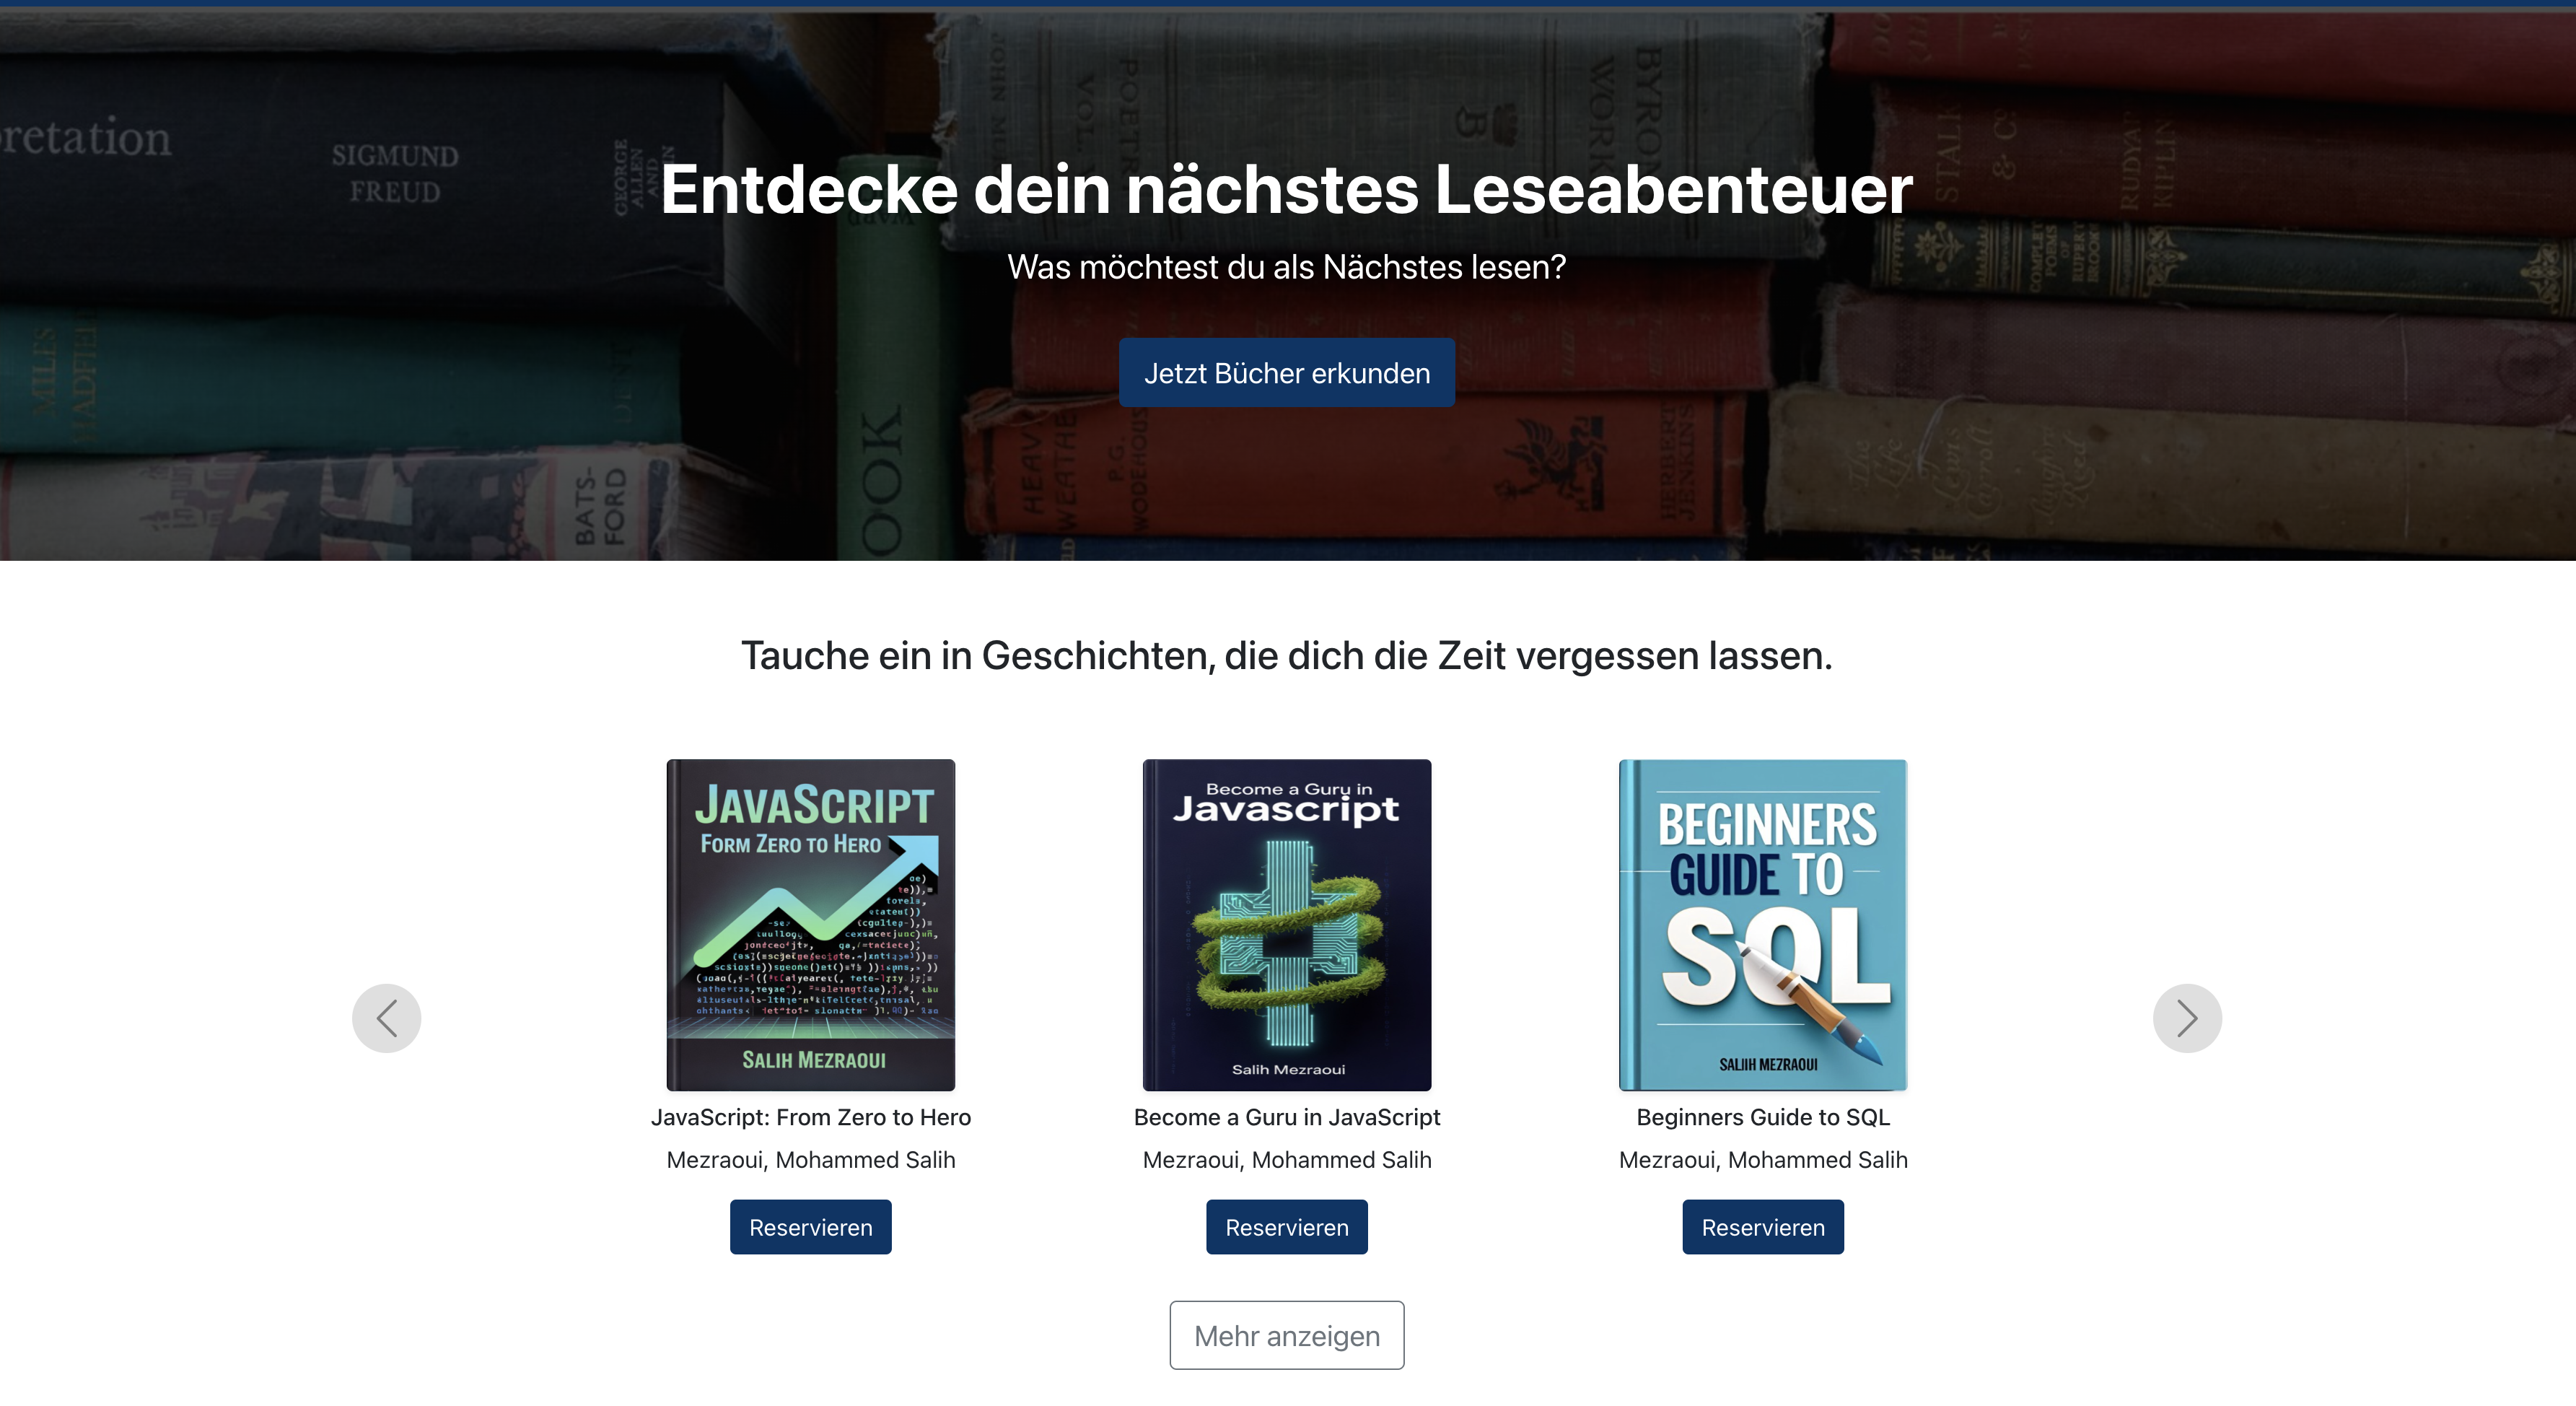
\includegraphics[width=1.0\textwidth]{images/UI-screenshots/Carousel_and_BookBrowser.png}%\subsection{Startseite (Main Page)}
	\caption{Karussell und Buch-Browser-Schaltfläche}
	\label{fig:Carousel_and_BookBrowser}%\subsubsection{Karussell (Carousel)}
\end{figure}

\section{Seitenübersicht}
Dieser Abschnitt gibt einen Überblick über zentrale Benutzeroberflächen der Anwendung, insbesondere die Buchsuchseite und die Buchdetailseite, und beschreibt deren wichtigste Funktionselemente.

\subsection{Buchsuche}

Die untenstehende Abbildung \ref{fig:Search-page} zeigt die Benutzeroberfläche der Suchseite. Sie enthält ein Suchfeld mit Schaltfläche sowie ein Dropdown-Menü zur Auswahl von Kategorien. Nutzer können entweder nach Stichwörtern, Kategorien oder einer Kombination aus beiden suchen. Die Suchergebnisse werden in paginierter Form dargestellt und beinhalten jeweils den Buchtitel, den Autor, eine Kurzbeschreibung, Verfügbarkeit sowie eine Schaltfläche zur Detailansicht des jeweiligen Buches.

\begin{figure}[H]
	\centering
	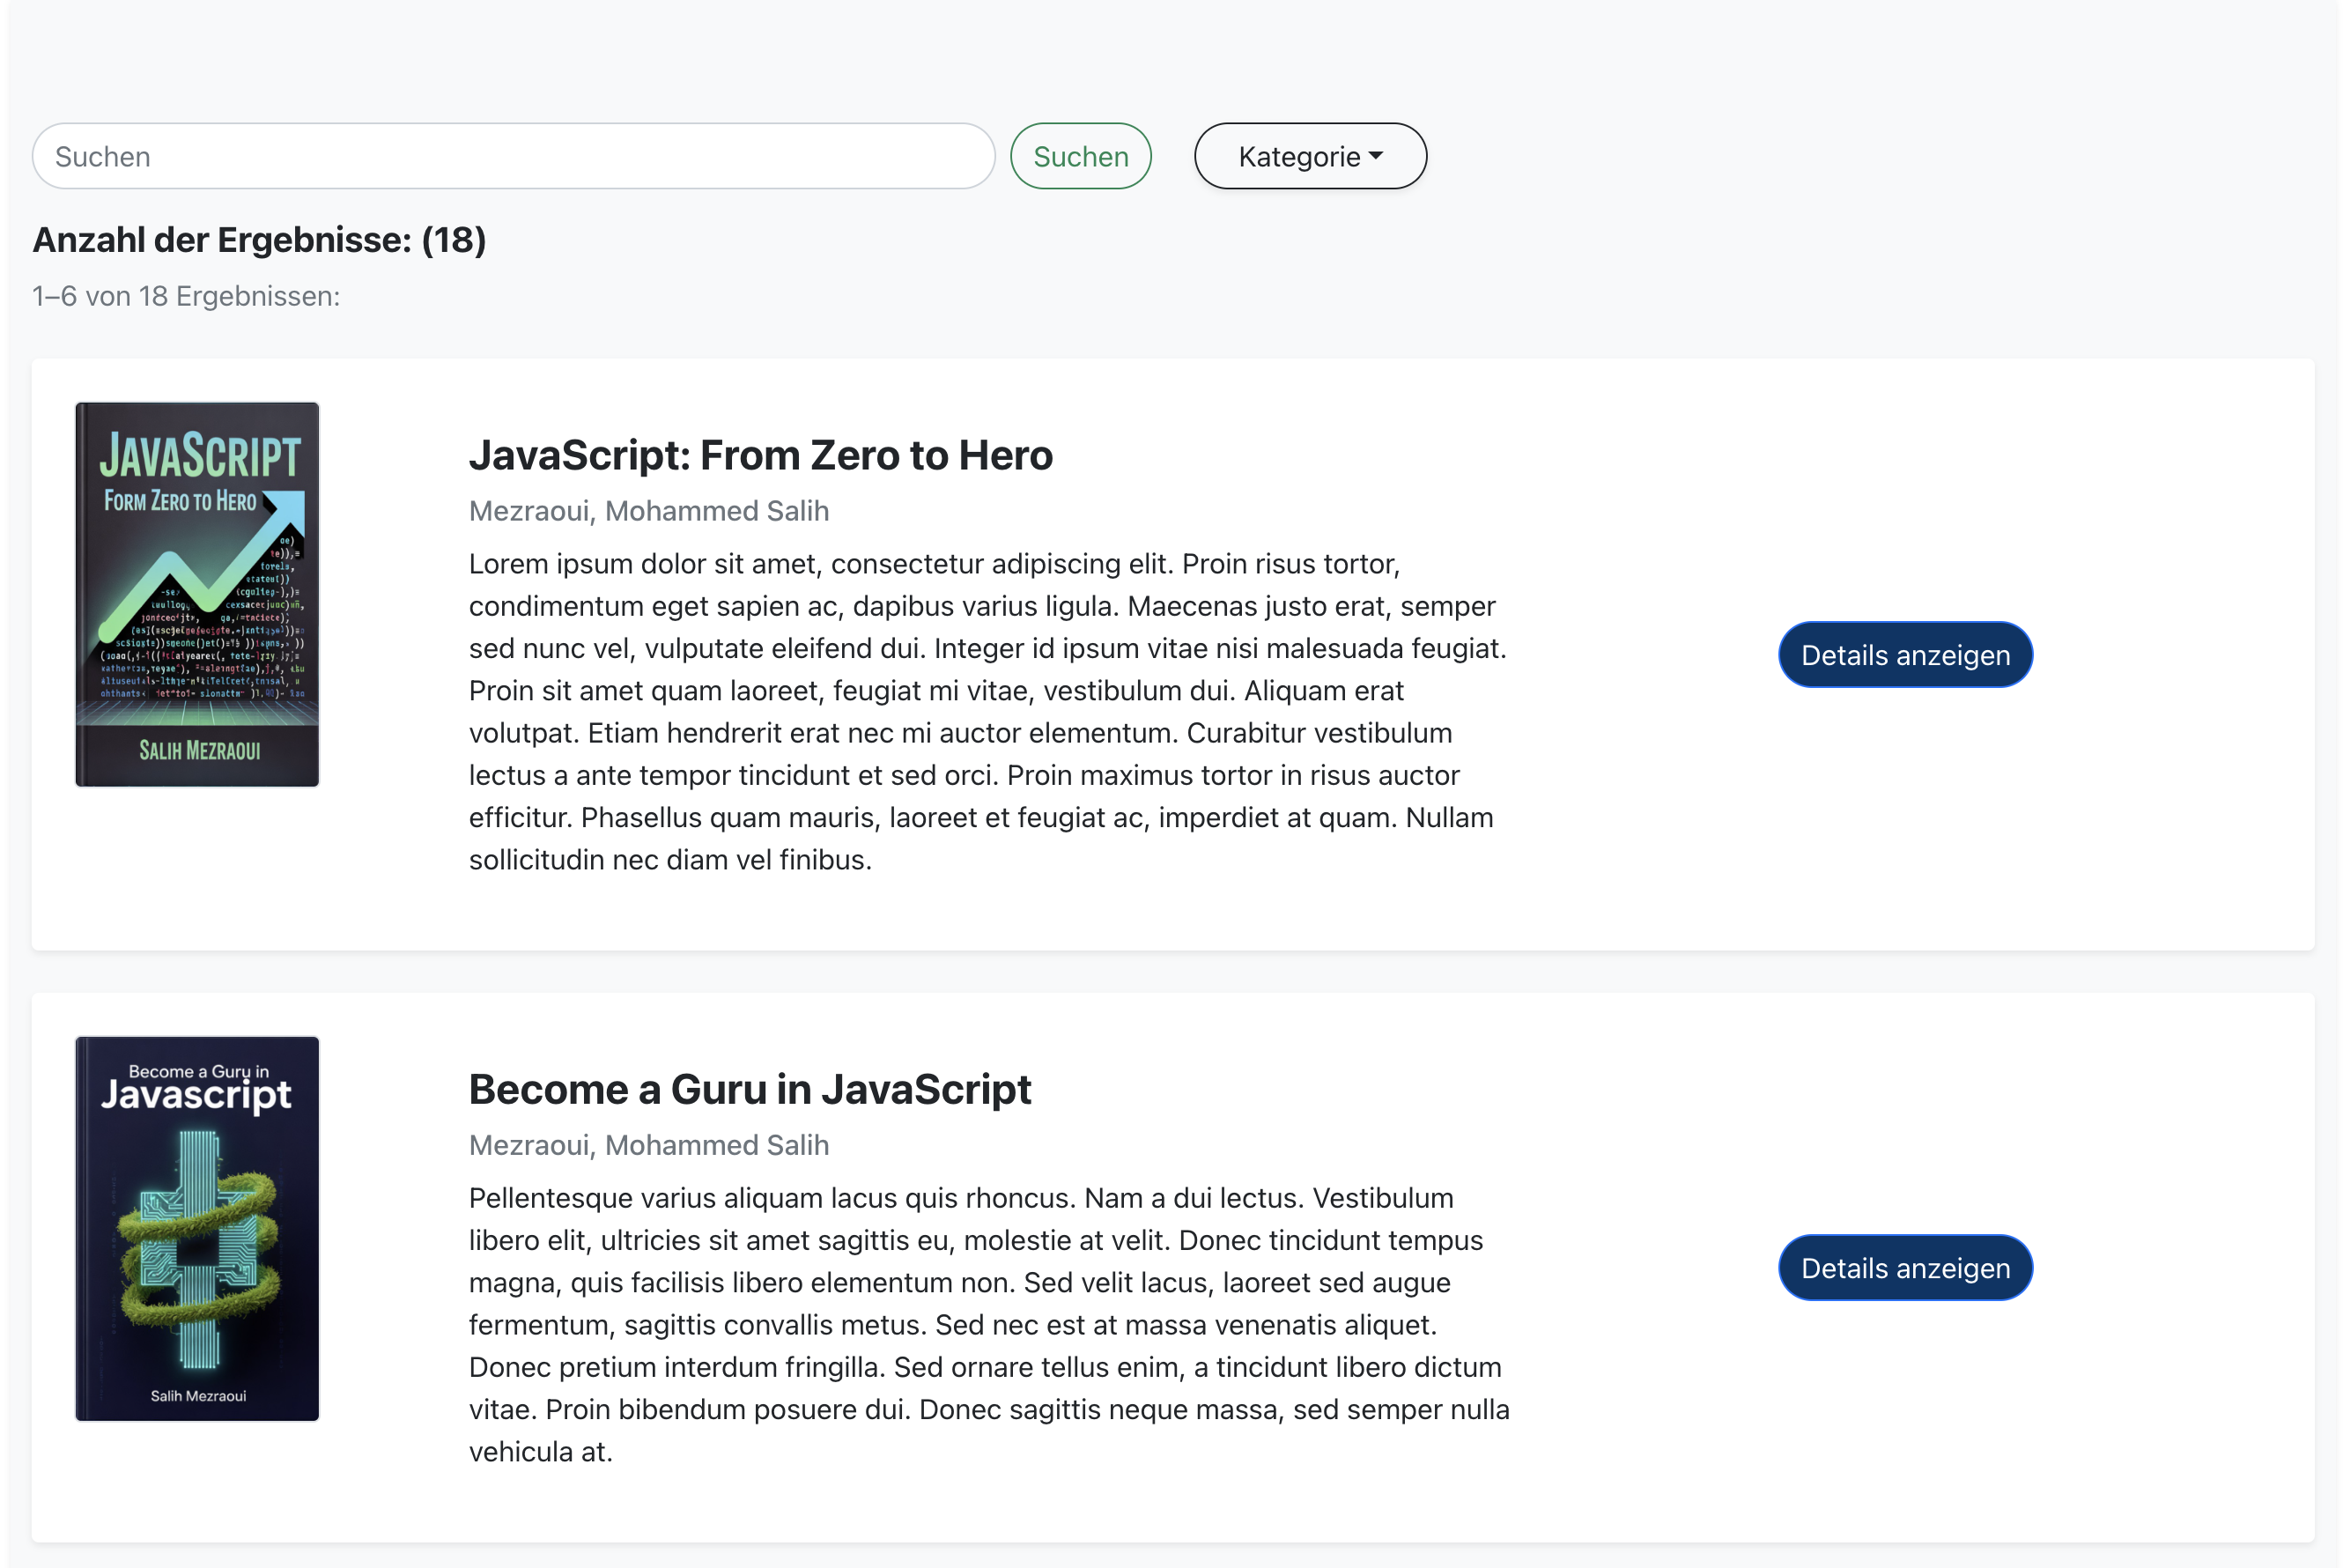
\includegraphics[width=1.0\textwidth]{images/UI-screenshots/Search-page.png}%\subsection{Startseite (Main Page)}
	\caption{Benutzeroberfläche der Suchseite}
	\label{fig:Search-page}
\end{figure}

\subsection{Buchseite}
Die untenstehende Abbildung  \ref{fig:Book-page} zeigt die Benutzeroberfläche der Buchseite. 

\begin{figure}[H]
	\centering
	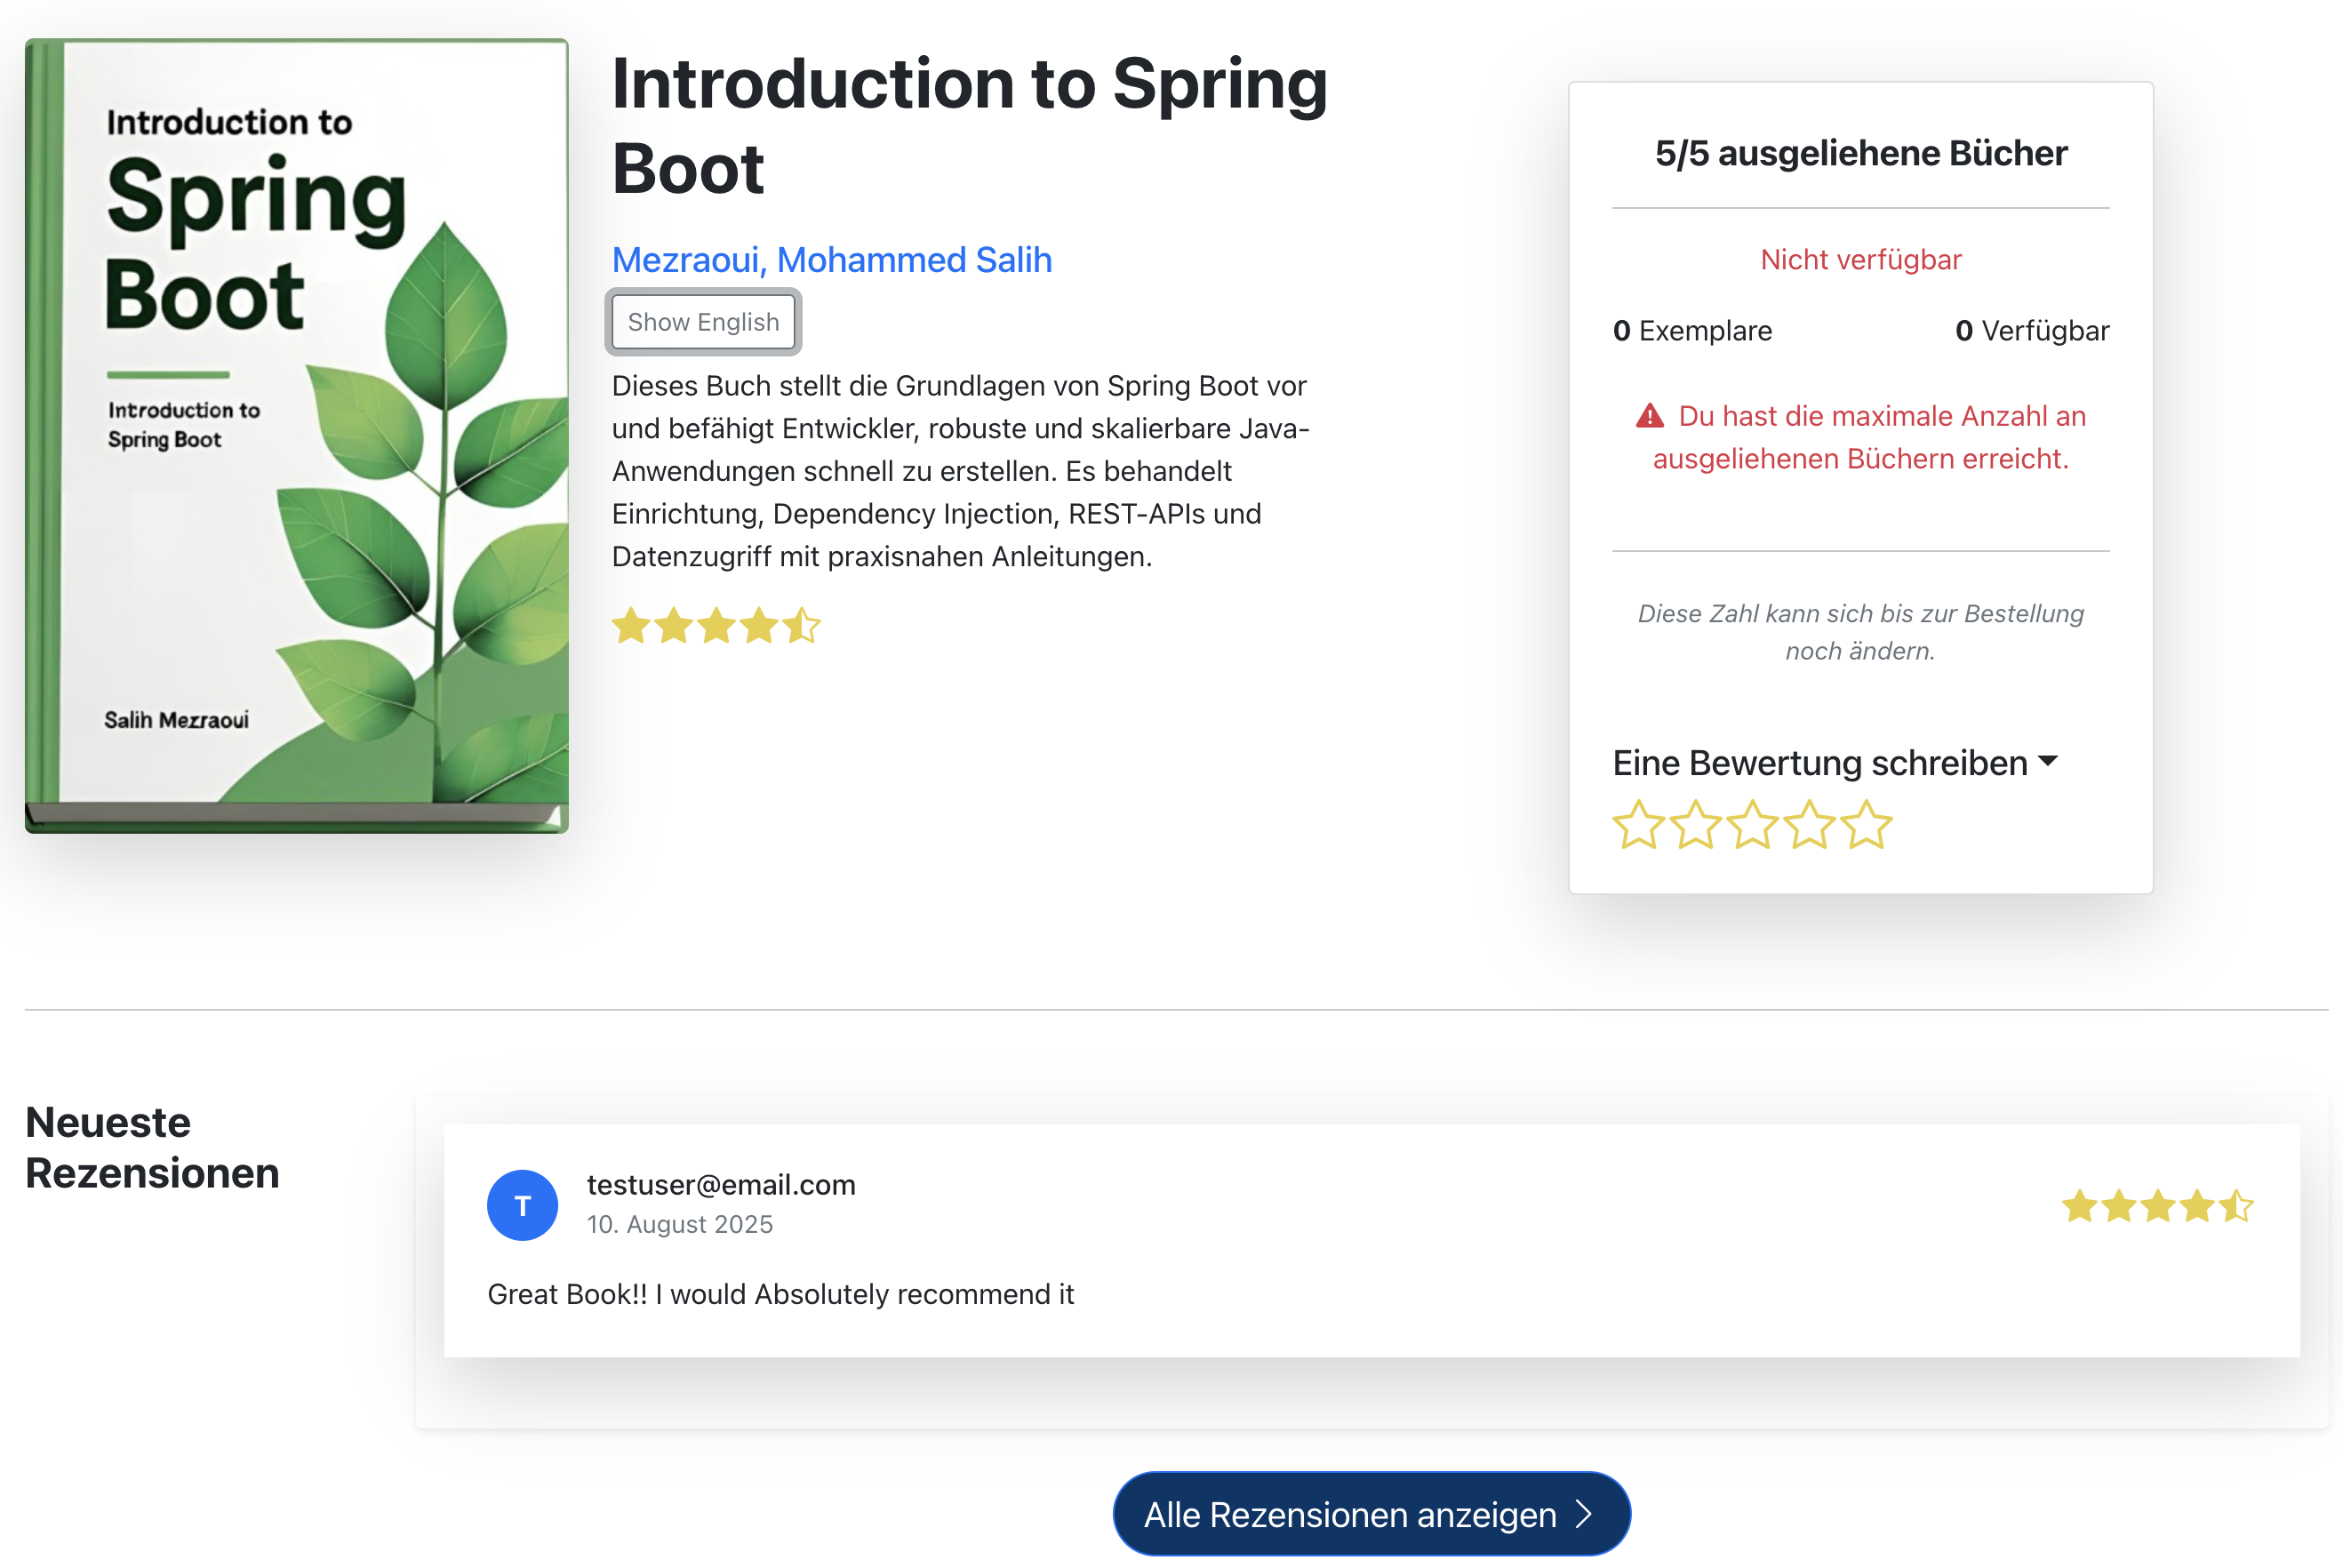
\includegraphics[width=1.0\textwidth]{images/UI-screenshots/Book-Page.png}
	\caption{Benutzeroberfläche der Buchseite}
	\label{fig:Book-page}
\end{figure}

\noindent Die Buchdetailseite stellt umfassende Informationen zu einem einzelnen Buch bereit. Sie zeigt das Buchcover, den Titel sowie den Autor an und bietet eine Buchbeschreibung, bei der zwischen deutscher und englischer Sprache gewechselt werden kann, unabhängig von der gewählten Sprache der Anwendung. Zudem enthält die Seite ein Bewertungssystem zur Anzeige der durchschnittlichen Nutzerbewertung. Auf der rechten Seitenleiste werden Informationen wie die Anzahl der vom aktuellen Benutzer ausgeliehenen Exemplare, die Anzahl der derzeit verfügbaren Exemplare sowie die Gesamtanzahl der im Bestand befindlichen Exemplare angezeigt. Zusätzlich bietet die Seite eine Übersicht der Nutzerbewertungen zum Buch sowie einen Link zur vollständigen Liste aller Reviews.

\section{Bibliotheksaktivität}
In diesem Abschnitt werden die Funktionen zur Verwaltung aktueller und vergangener Ausleihen dargestellt.

\subsection{Ausleihen}
Die untenstehende Abbildung \ref{fig:Loans-Page} zeigt das Design der aktuellen \texttt{Ausleihen} Seite. 

\begin{figure}[H]
	\centering
	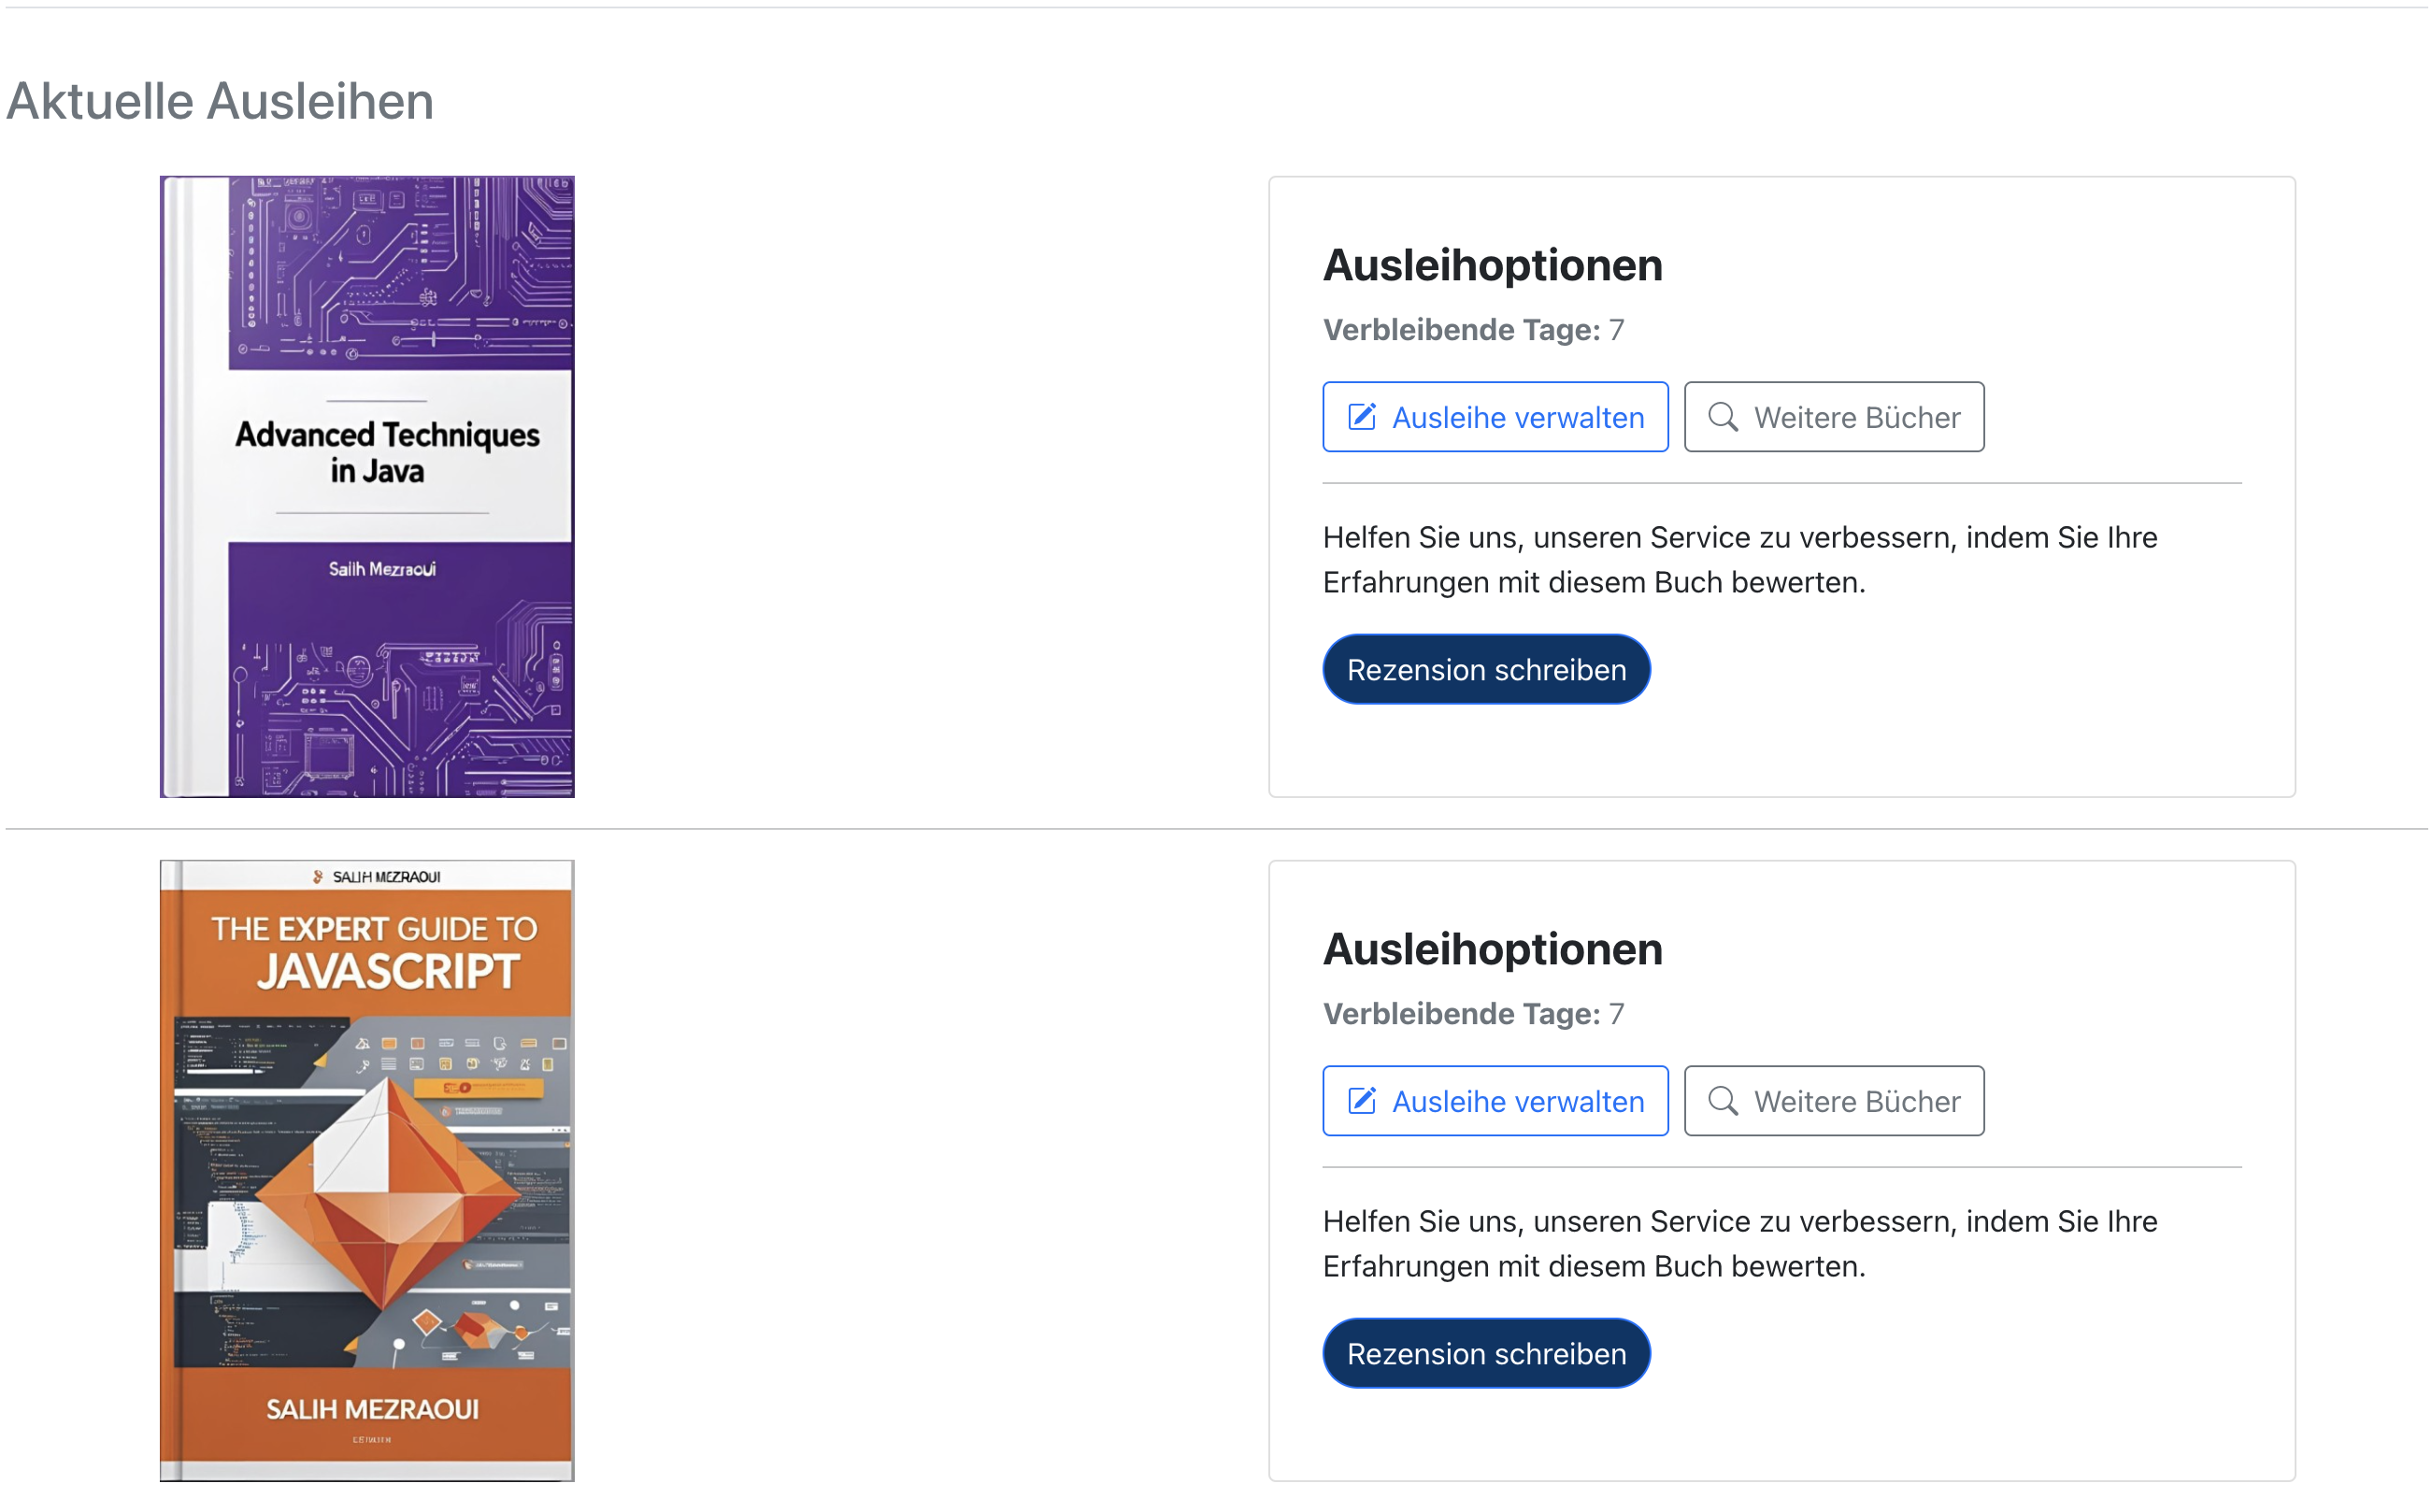
\includegraphics[width=1.0\textwidth]{images/UI-screenshots/Loans-Page.png}
	\caption{Benutzeroberfläche der Ausleihseite}
	\label{fig:Loans-Page}
\end{figure}

\noindent Die Ausleiheseite ermöglicht es Nutzenden, ihre aktuell ausgeliehenen Bücher zu verwalten. Sie zeigt eine Liste aller ausgeliehenen Bücher an und gibt für jedes Buch die verbleibenden Tage bis zur Rückgabe an. Für jedes Buch stehen Verwaltungsoptionen wie die Rückgabe oder die Verlängerung der Leihfrist zur Verfügung. Zusätzlich enthält die Seite eine Schaltfläche zur Suche nach weiteren Büchern sowie einen Link, um eine Rezension für das jeweilige Buch zu verfassen.

\subsection{Ausleihhistorie}
Die untenstehende Abbildung \ref{fig:Loans-History-Page} zeigt das Design der Seite \texttt{Ausleihverlauf}. Diese Seite enthält die Historie der vom Nutzer ausgeliehenen Bücher, einschließlich des Ausleih- und Rückgabedatums.

\begin{figure}[H]
	\centering
	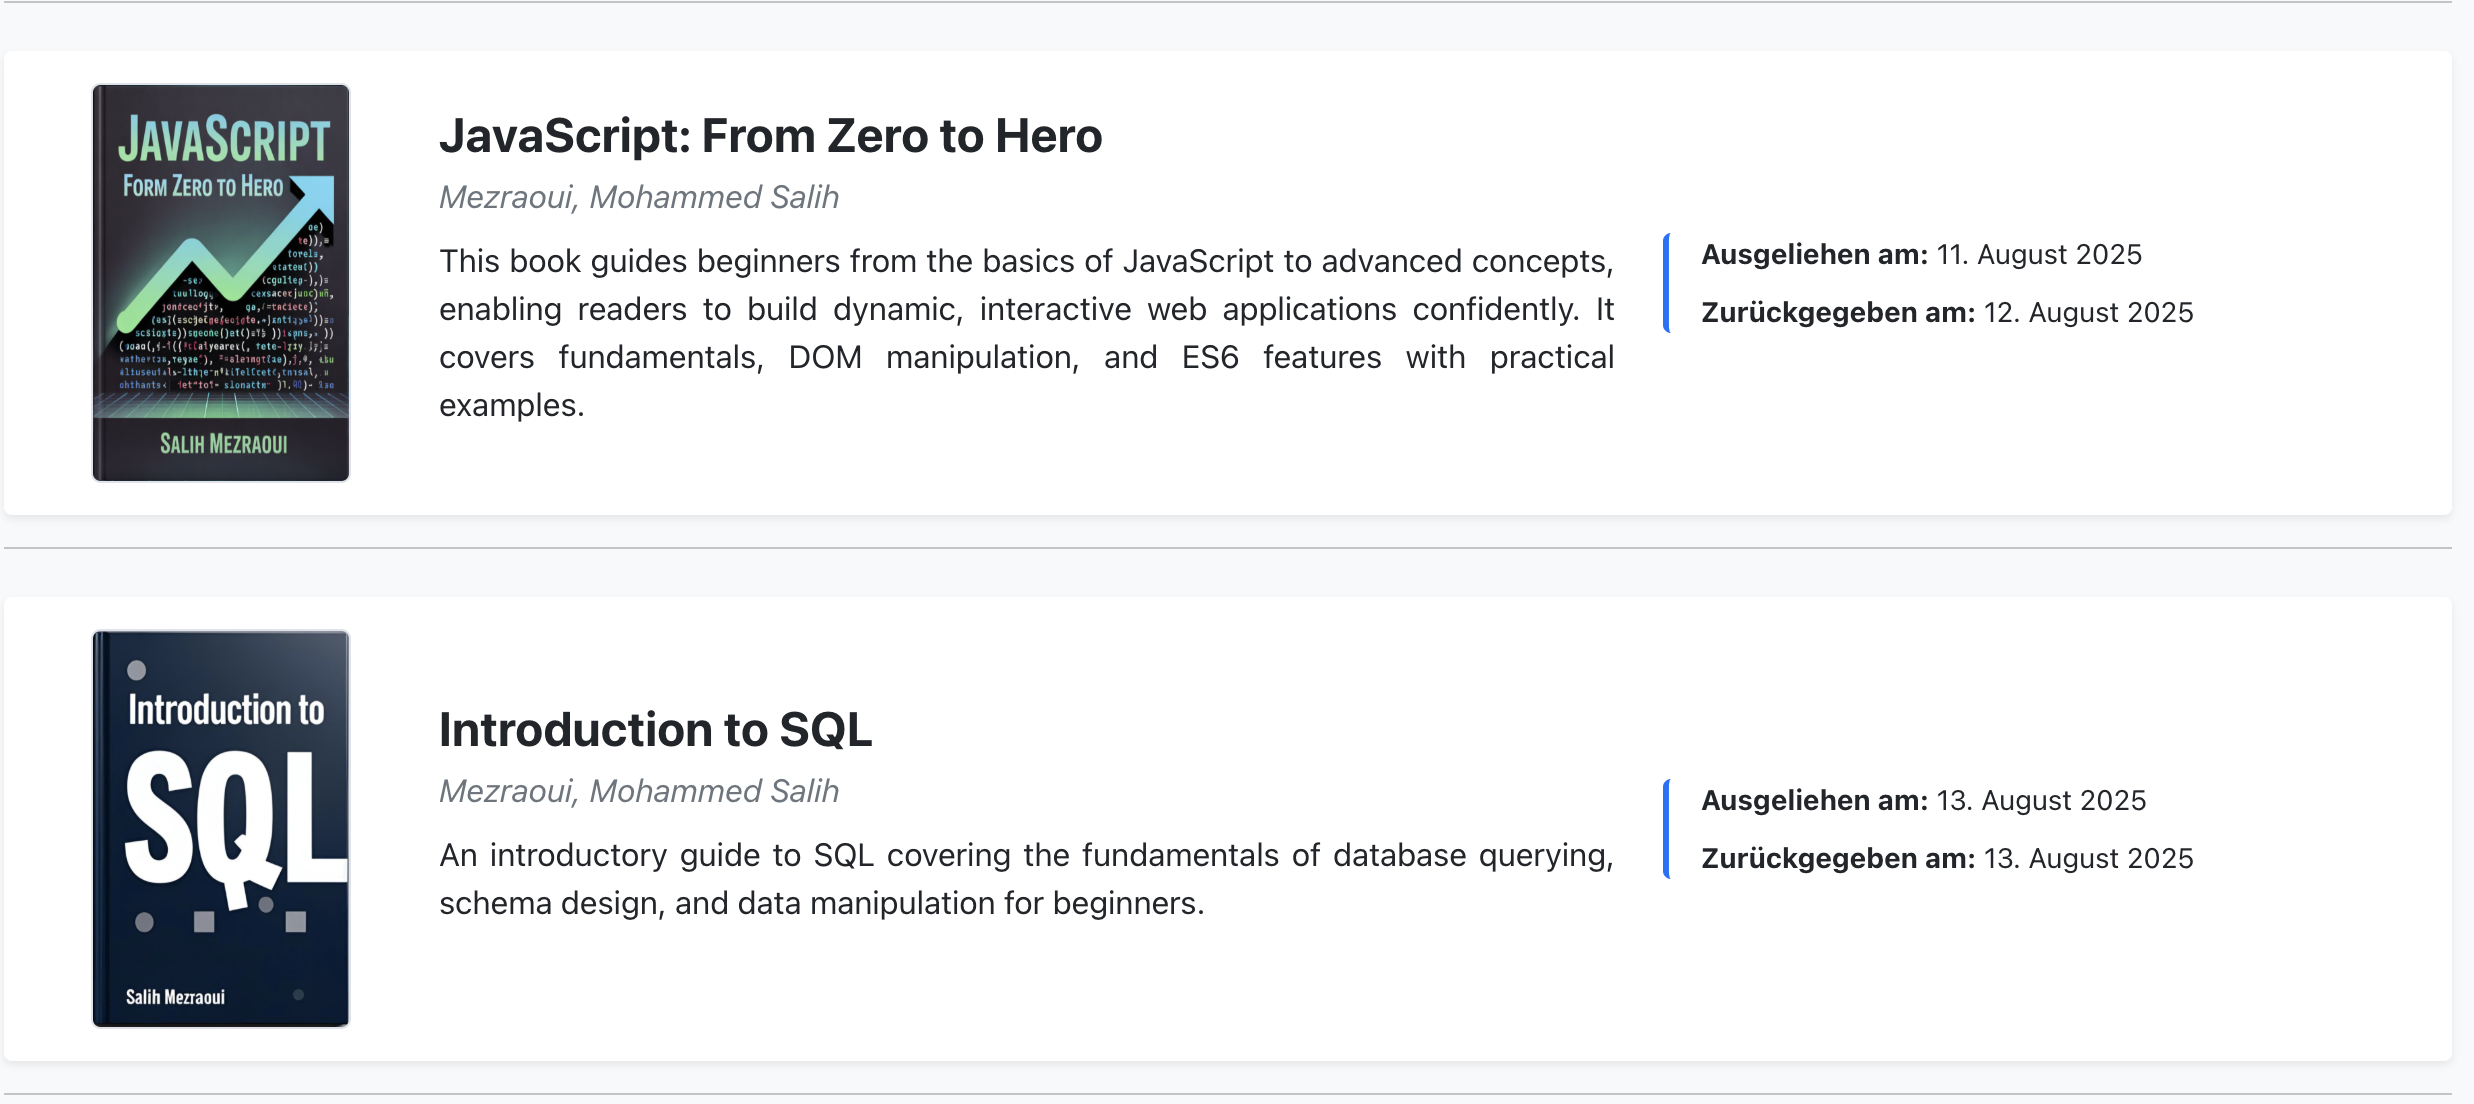
\includegraphics[width=1.0\textwidth]{images/UI-screenshots/Loans-History.png}
	\caption{Benutzeroberfläche der Ausleihverlaufsseite}%\subsection{Bibliotheksservice (Library Service)}
	\label{fig:Loans-History-Page}
\end{figure}

\section{Bibliotheksdienste}
In diesem Abschnitt werden die Bibliotheksdienste vorgestellt, insbesondere die Benutzeroberfläche zur Übermittlung von Anfragen sowie der persönliche Nachrichtenverlauf mit den jeweiligen Antworten.

\noindent Die folgende Abbildung \ref{fig:Message-Send} zeigt die Benutzeroberfläche, über die Benutzer einzelne Anfragen oder Nachrichten an die Administratoren der Bibliothek senden können.

\begin{figure}[H]
	\centering
	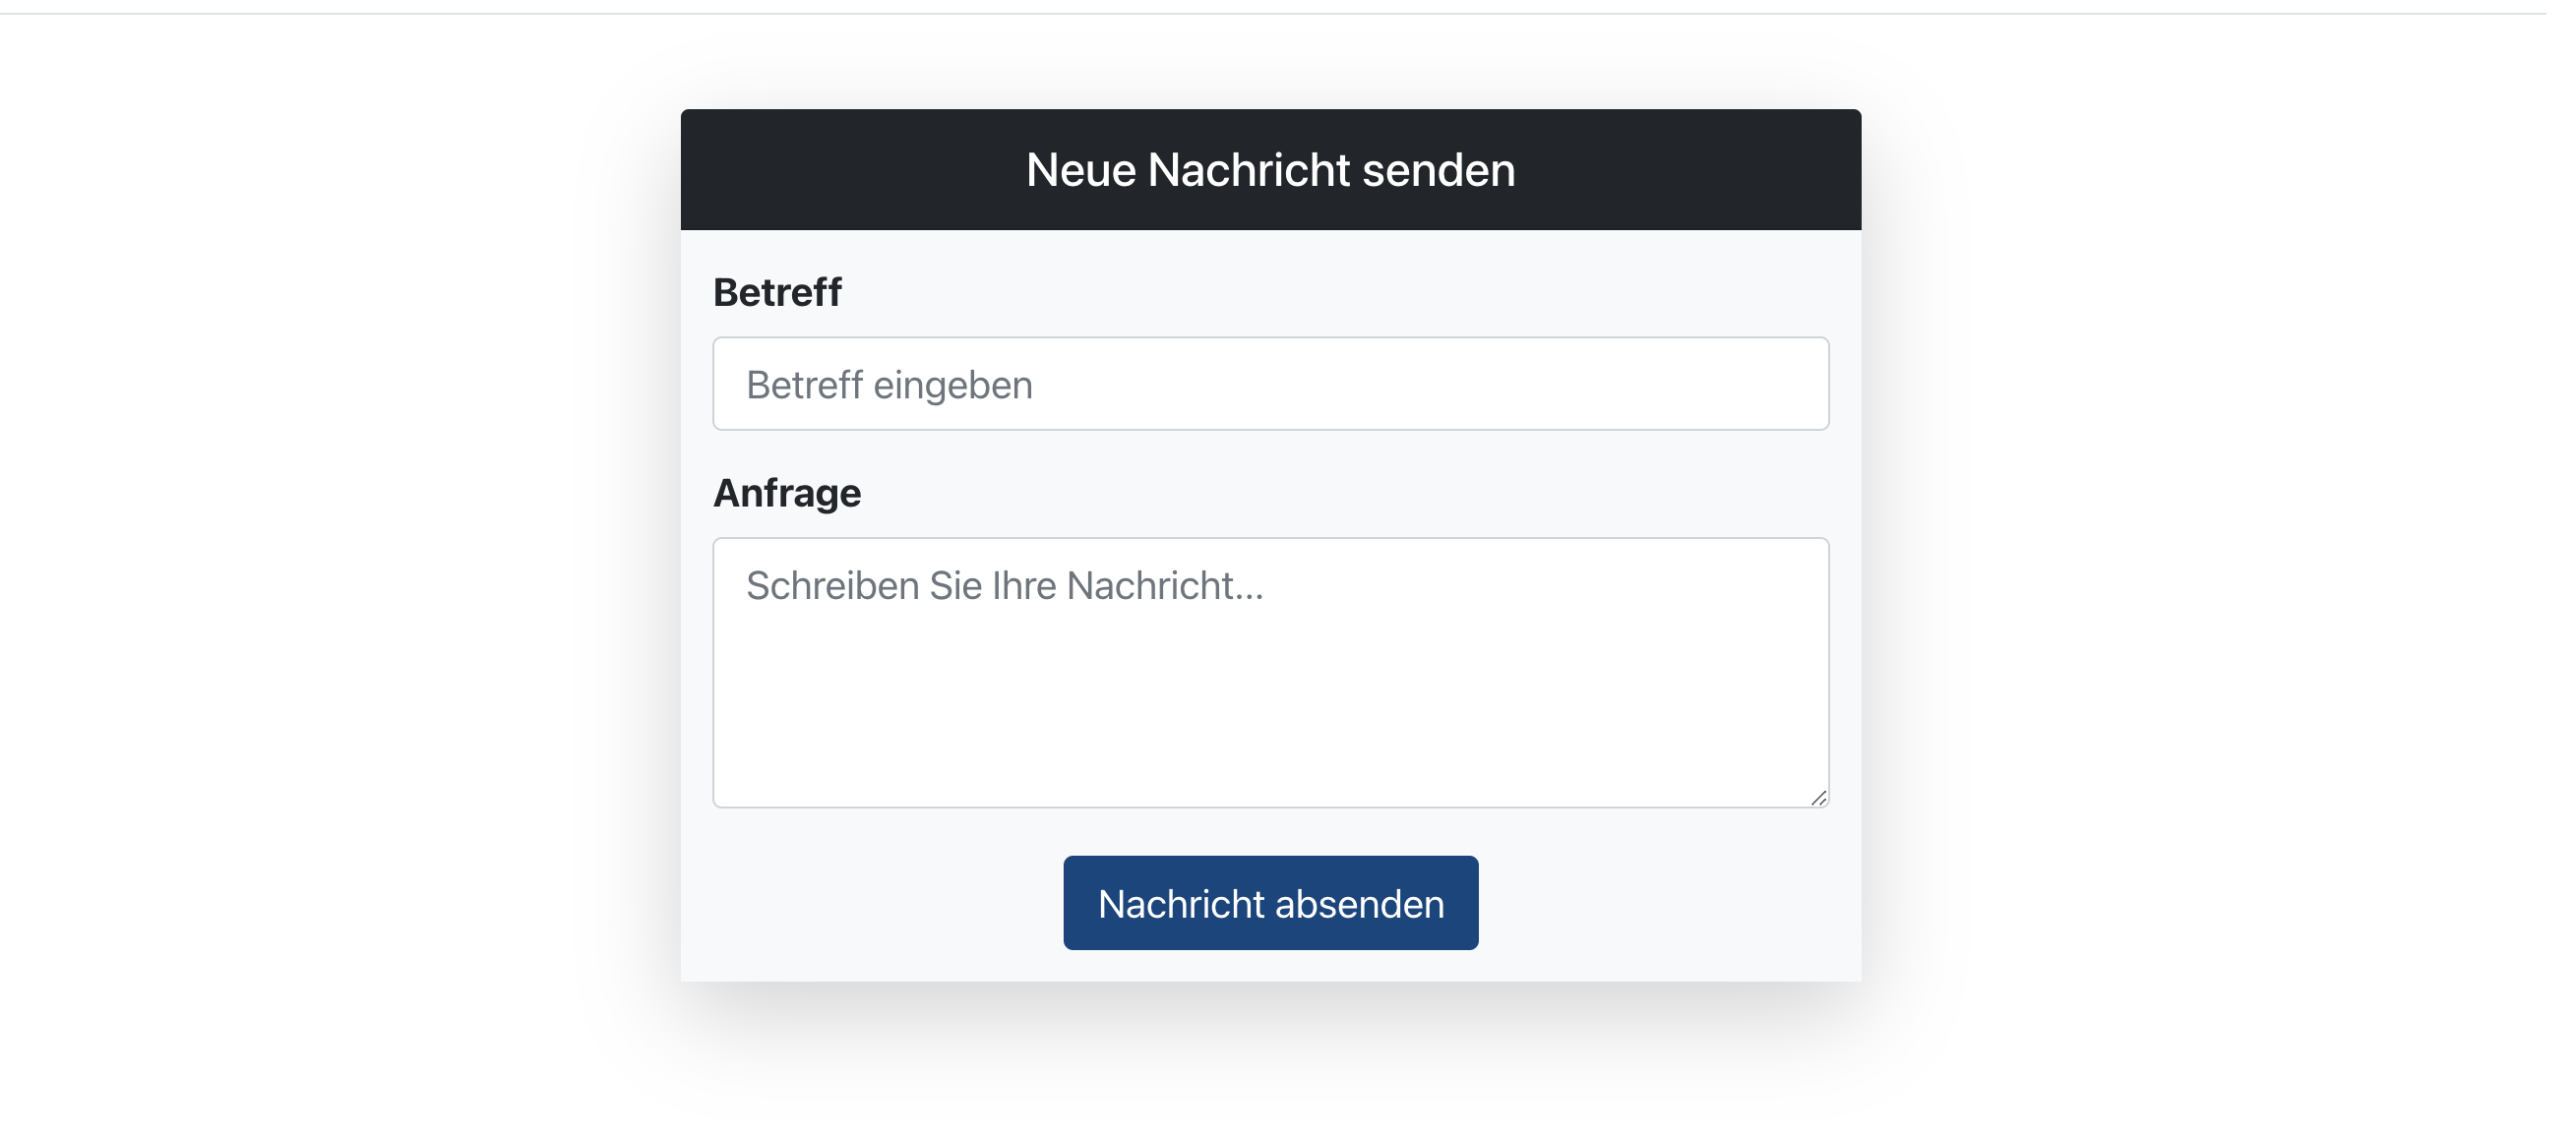
\includegraphics[width=0.9\textwidth]{images/UI-screenshots/Message-Send.png}
	\caption{Benutzeroberfläche zum Versenden von Anfragen}
	\label{fig:Message-Send}
\end{figure}

\noindent Die Abbildung \ref{fig:Messages-History} veranschaulicht den Verlauf sämtlicher ausgetauschter Nachrichten, einschließlich der gestellten Fragen und der dazugehörigen Antworten.

\begin{figure}[H]
	\centering
	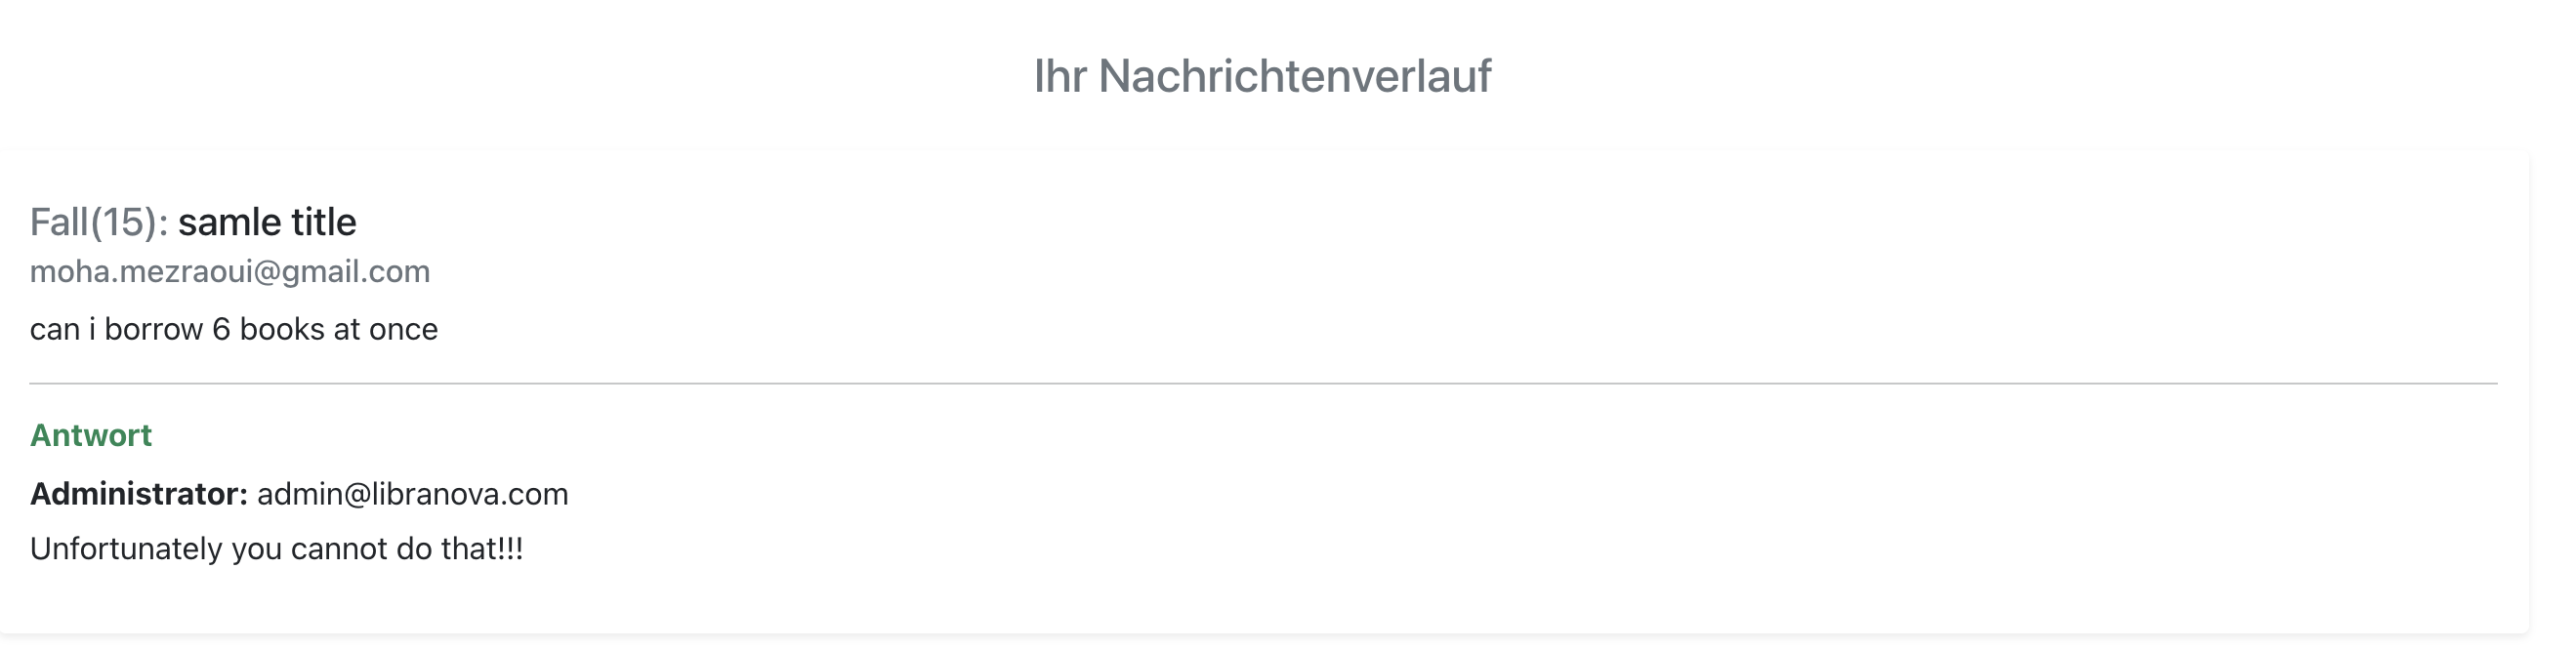
\includegraphics[width=1.0\textwidth]{images/UI-screenshots/Messages-History.png}
	\caption{Nachrichtenverlauf zwischen Nutzer und Bibliothek}
	\label{fig:Messages-History}
\end{figure}

\section{Bezahlungsseite}

In diesem Abschnitt wird die Benutzeroberfläche zur Verwaltung von Zahlungsinformationen und offenen Gebühren vorgestellt.

\noindent Abbildung \ref{fig:Outstanding-payment} zeigt das Layout, das angezeigt wird, wenn ein Benutzer ausstehende Zahlungen zu begleichen hat. 

\begin{figure}[H]
	\centering
	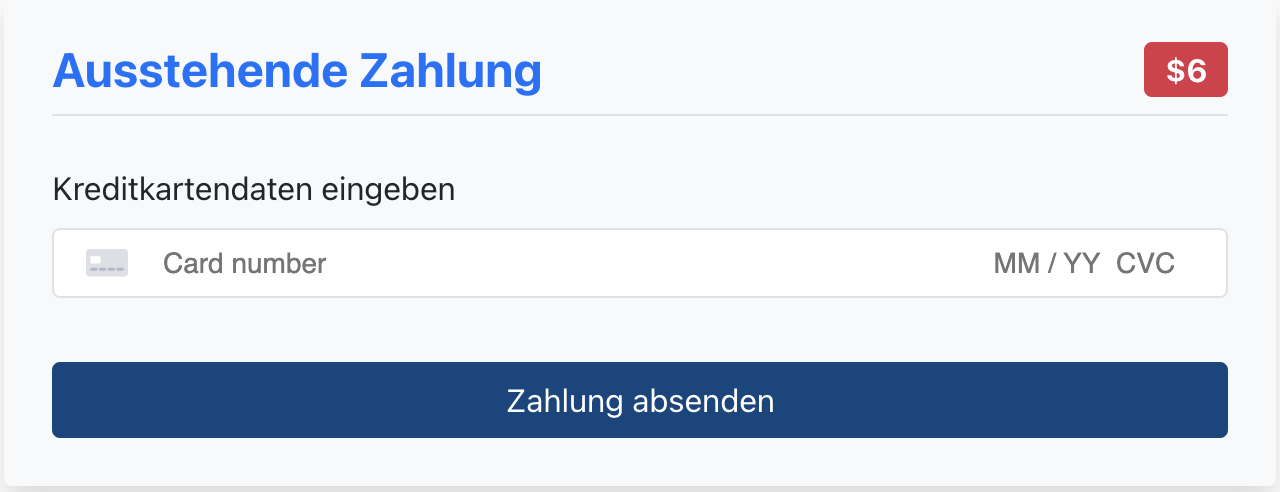
\includegraphics[width=1.0\textwidth]{images/UI-screenshots/Outstanding-payment.png}
	\caption{Benutzeroberfläche bei ausstehenden Zahlungen}
	\label{fig:Outstanding-payment}
\end{figure}

\noindent Wenn keine offenen Gebühren vorliegen, wird dem Nutzer die in Abbildung \ref{fig:No-Payment} dargestellte Ansicht präsentiert. Sie bestätigt, dass derzeit keine Zahlungen erforderlich sind.

\begin{figure}[H]
	\centering
	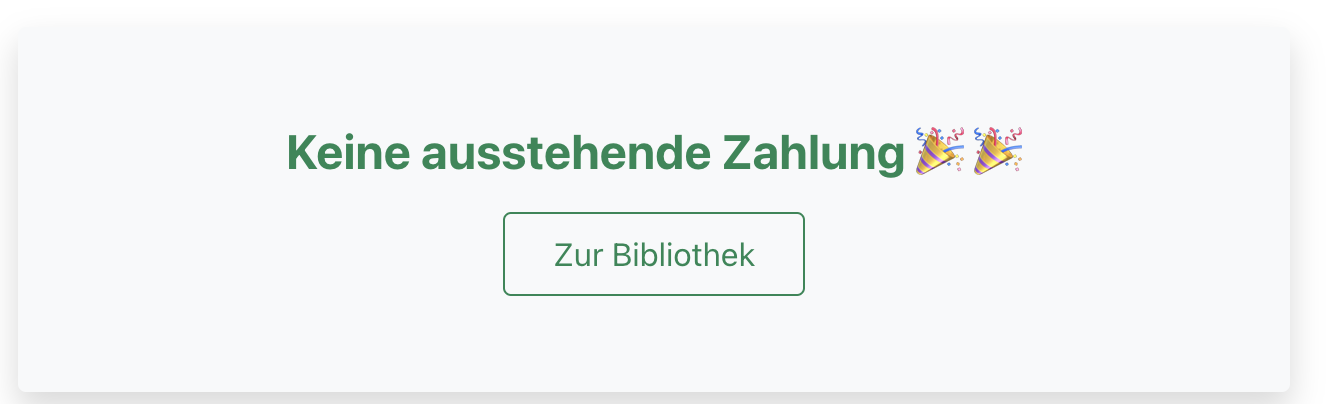
\includegraphics[width=1.0\textwidth]{images/UI-screenshots/No-Payment.png}
	\caption{Benutzeroberfläche bei keinen offenen Zahlungen}
	\label{fig:No-Payment}
\end{figure}

\section{Admin-Bereich}

Der Admin-Bereich bietet eine dedizierte Oberfläche zur Verwaltung der Bibliotheksressourcen und zur Interaktion mit Benutzeranfragen. In diesem Abschnitt werden die Verwaltungsfunktionen dargestellt, die einem Administrator zur Verfügung stehen.

\subsection{Neues Buch hinzufügen}
\noindent Die erste Funktion (siehe \ref{fig:Add-New-Book}) ermöglicht es dem Administrator, neue Bücher in das System aufzunehmen. Hierzu gibt er relevante Informationen wie Titel, Autor, Kategorie, eine kurze Beschreibung sowie die Anzahl der verfügbaren Exemplare an. Zusätzlich kann ein Bild des Buchcovers hochgeladen werden. Nach dem Ausfüllen der Felder wird durch Klicken auf die Schaltfläche \textit{"Buch hinzufügen"} ein neuer Eintrag erstellt.
\begin{figure}[H]
	\centering
	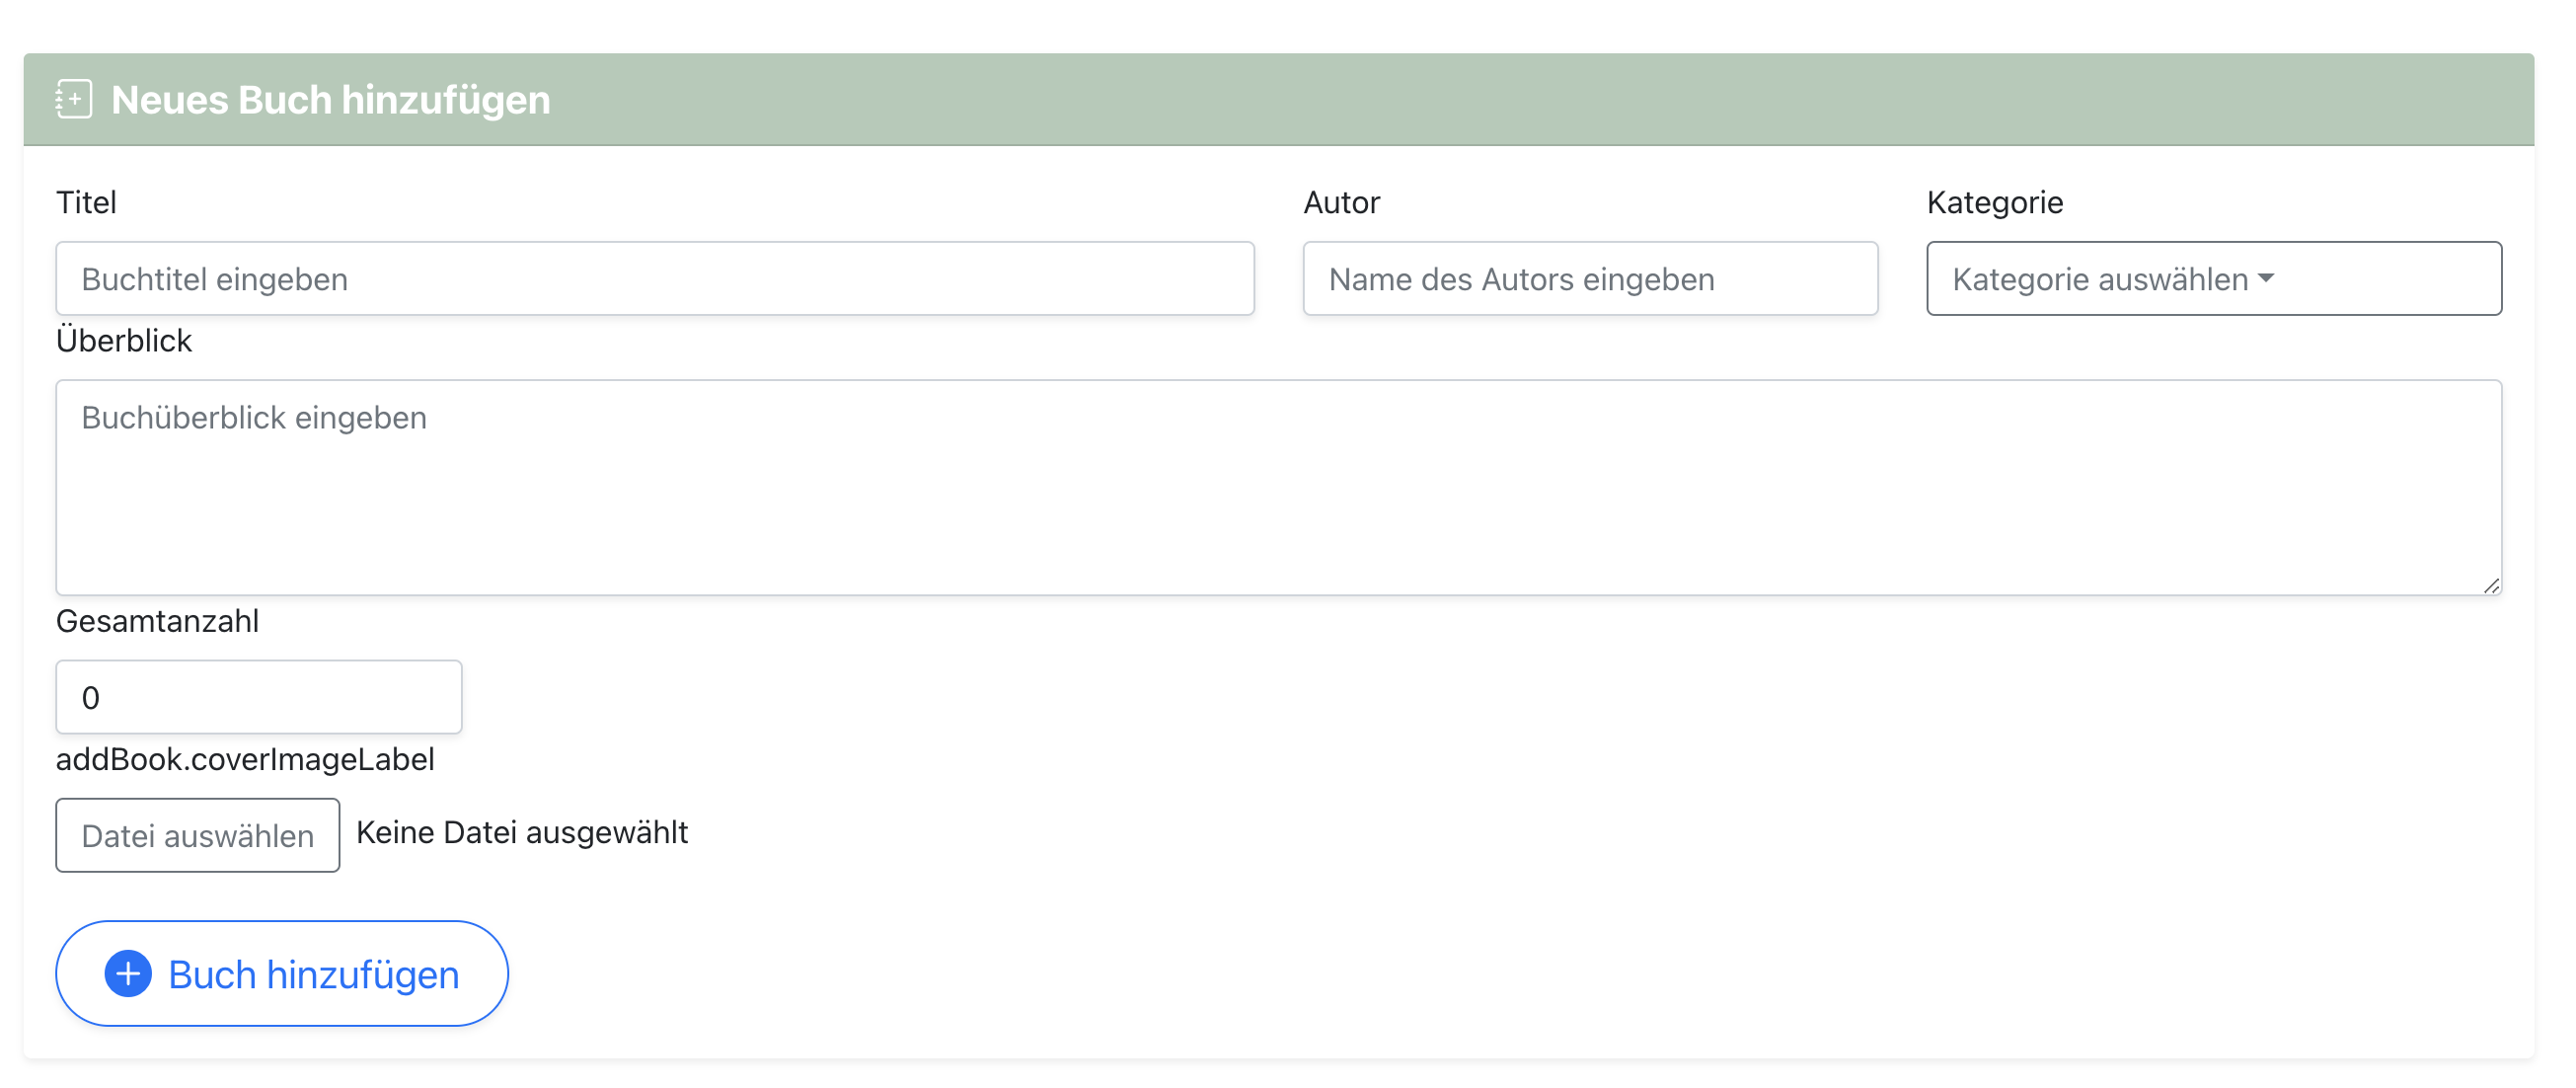
\includegraphics[width=1.0\textwidth]{images/UI-screenshots/Add-New-Book.png}
	\caption{Das Design zum Hinzufügen eines neuen Buches}
	\label{fig:Add-New-Book}
\end{figure}

\subsection{Bücher verwalten}

\noindent Der Administrator kann bestehende Bücher verwalten, indem er die Anzahl der verfügbaren Exemplare anpasst oder Bücher vollständig aus dem System entfernt. Die folgende Abbildung \ref{fig:Manage-Books} zeigt die Verwaltungsoberfläche, über die solche Änderungen vorgenommen werden können.

\begin{figure}[H]
	\centering
	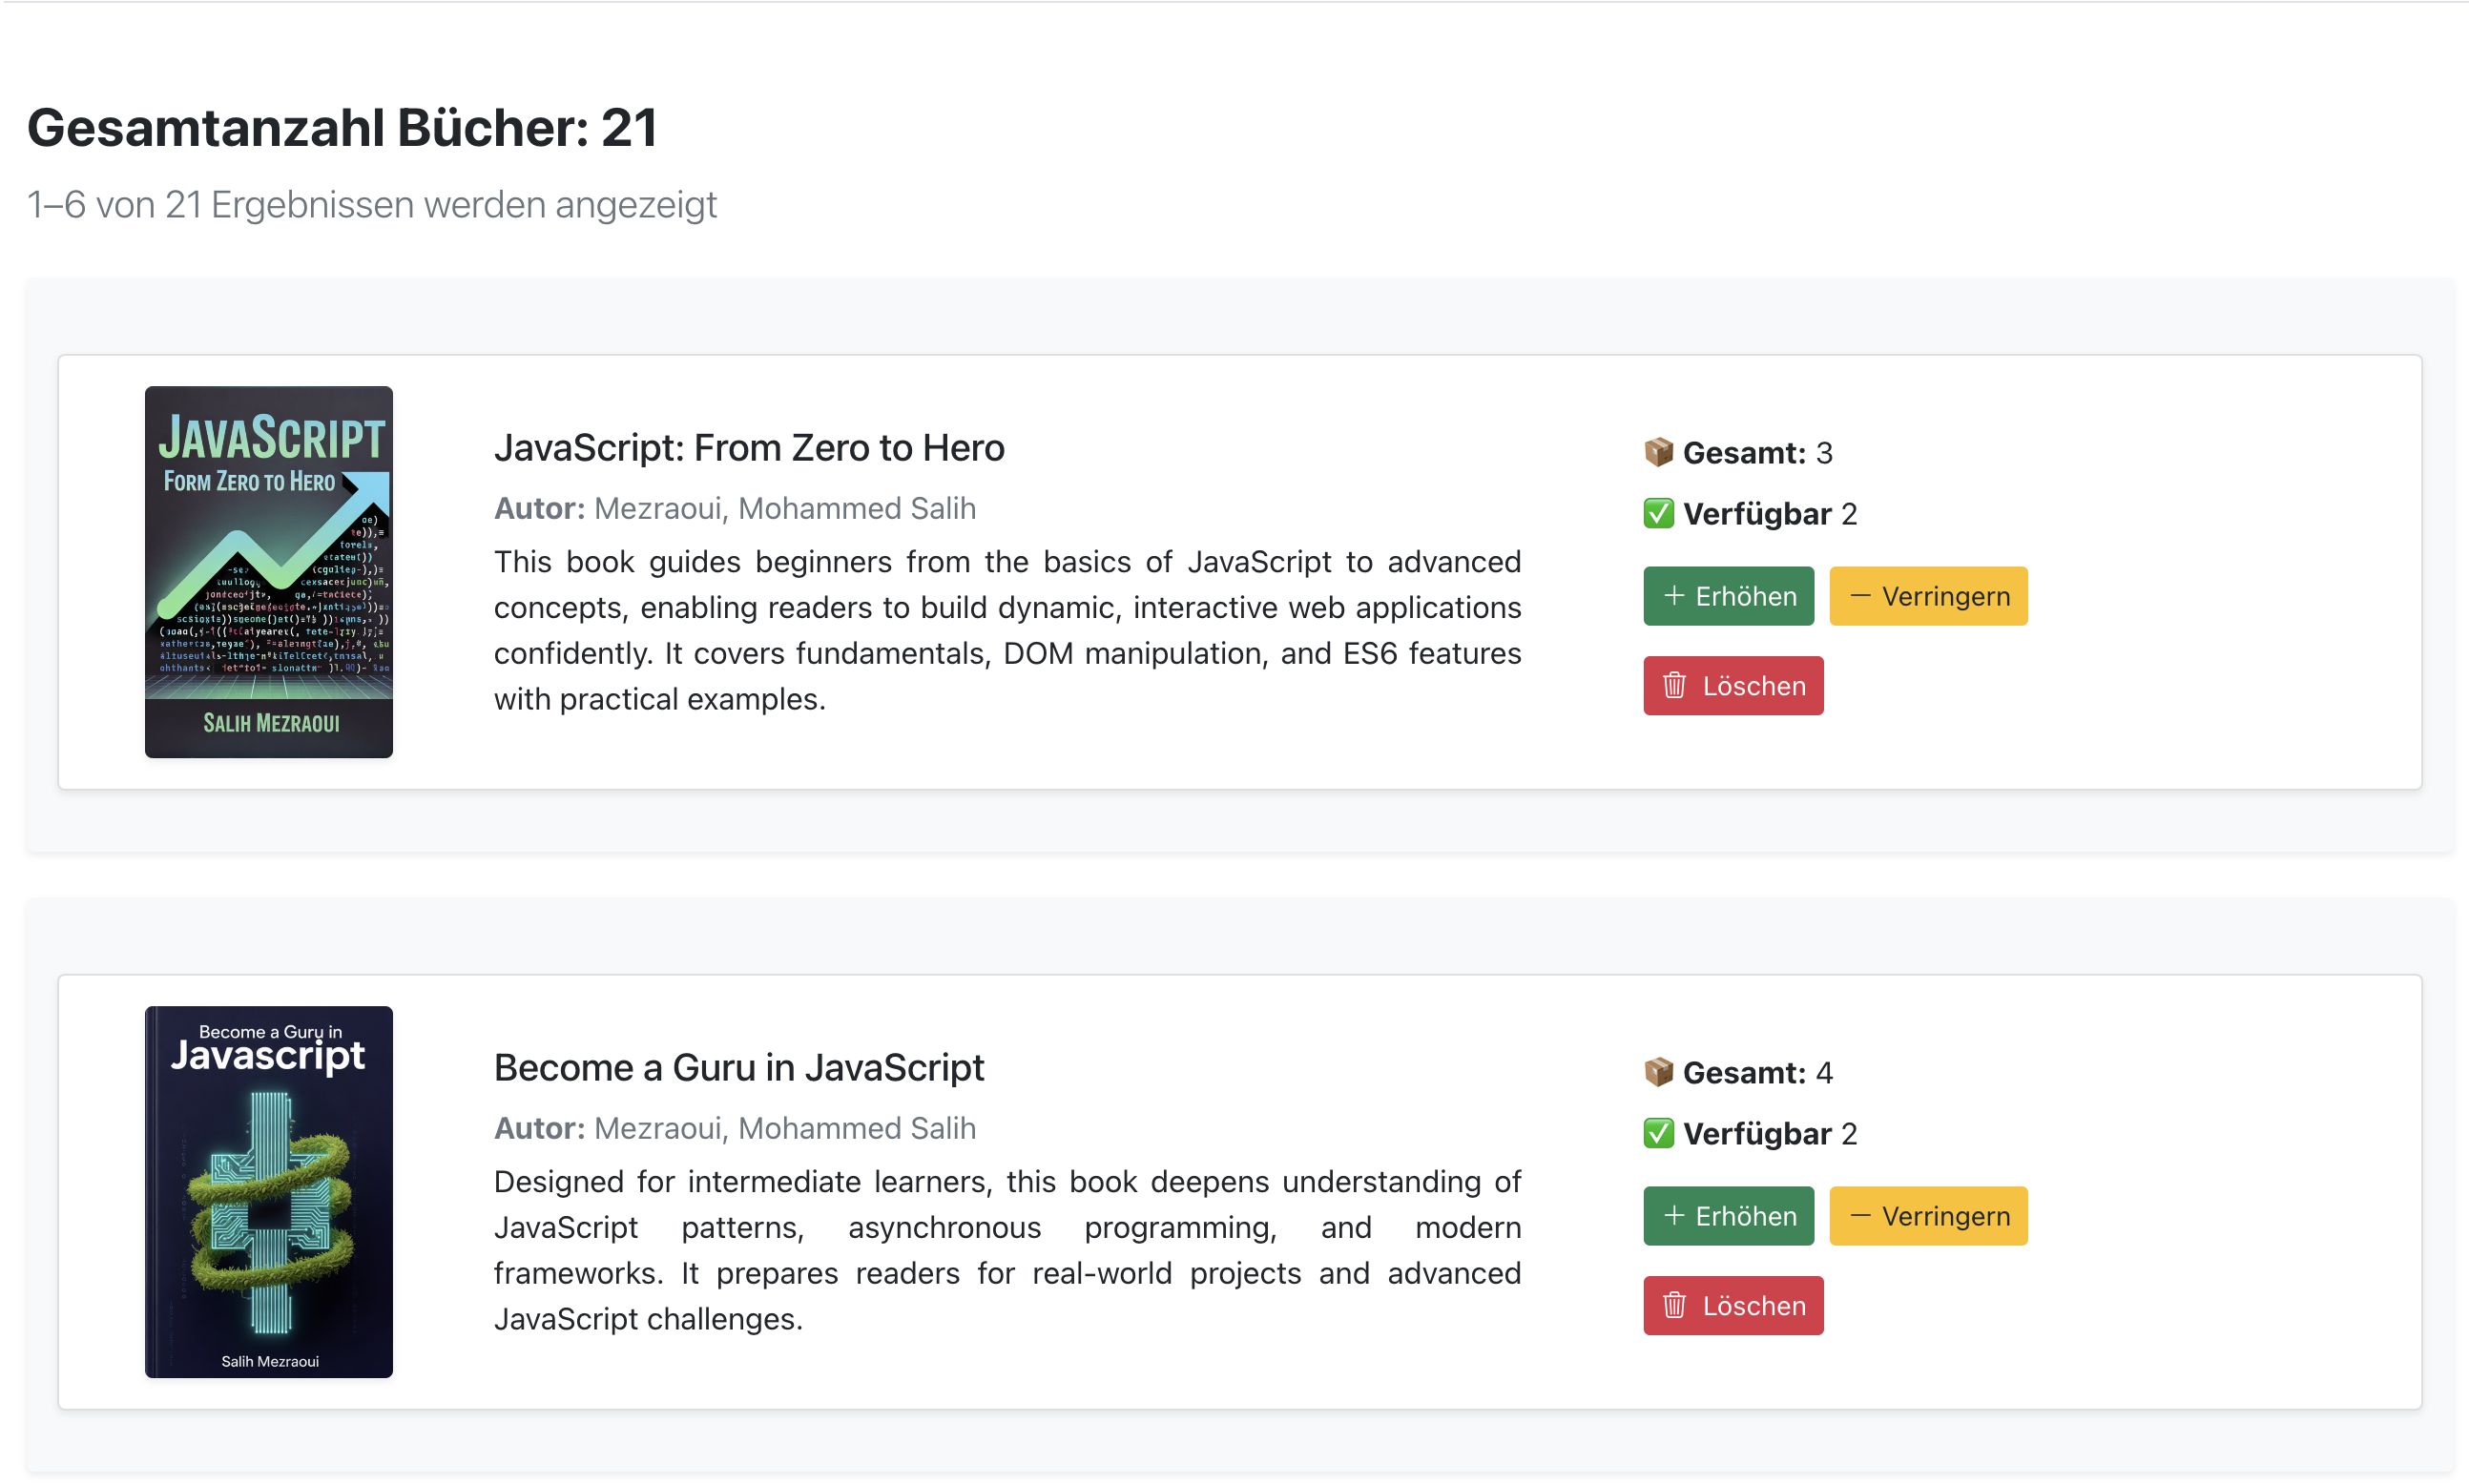
\includegraphics[width=1.0\textwidth]{images/UI-screenshots/Manage-Books.png}
	\caption{Das Design der Buchverwaltung}
	\label{fig:Manage-Books}
\end{figure}
\subsection{Nachrichten}

\noindent In diesem Bereich kann der Administrator auf Anfragen von Benutzern antworten. Die Benutzerfrage wird angezeigt und kann direkt über das vorgesehene Textfeld beantwortet werden. Eine Schaltfläche ermöglicht das Senden der Antwort. Die Abbildung \ref{fig:Messages-Responses} zeigt die zugehörige Benutzeroberfläche.

\begin{figure}[H]
	\centering
	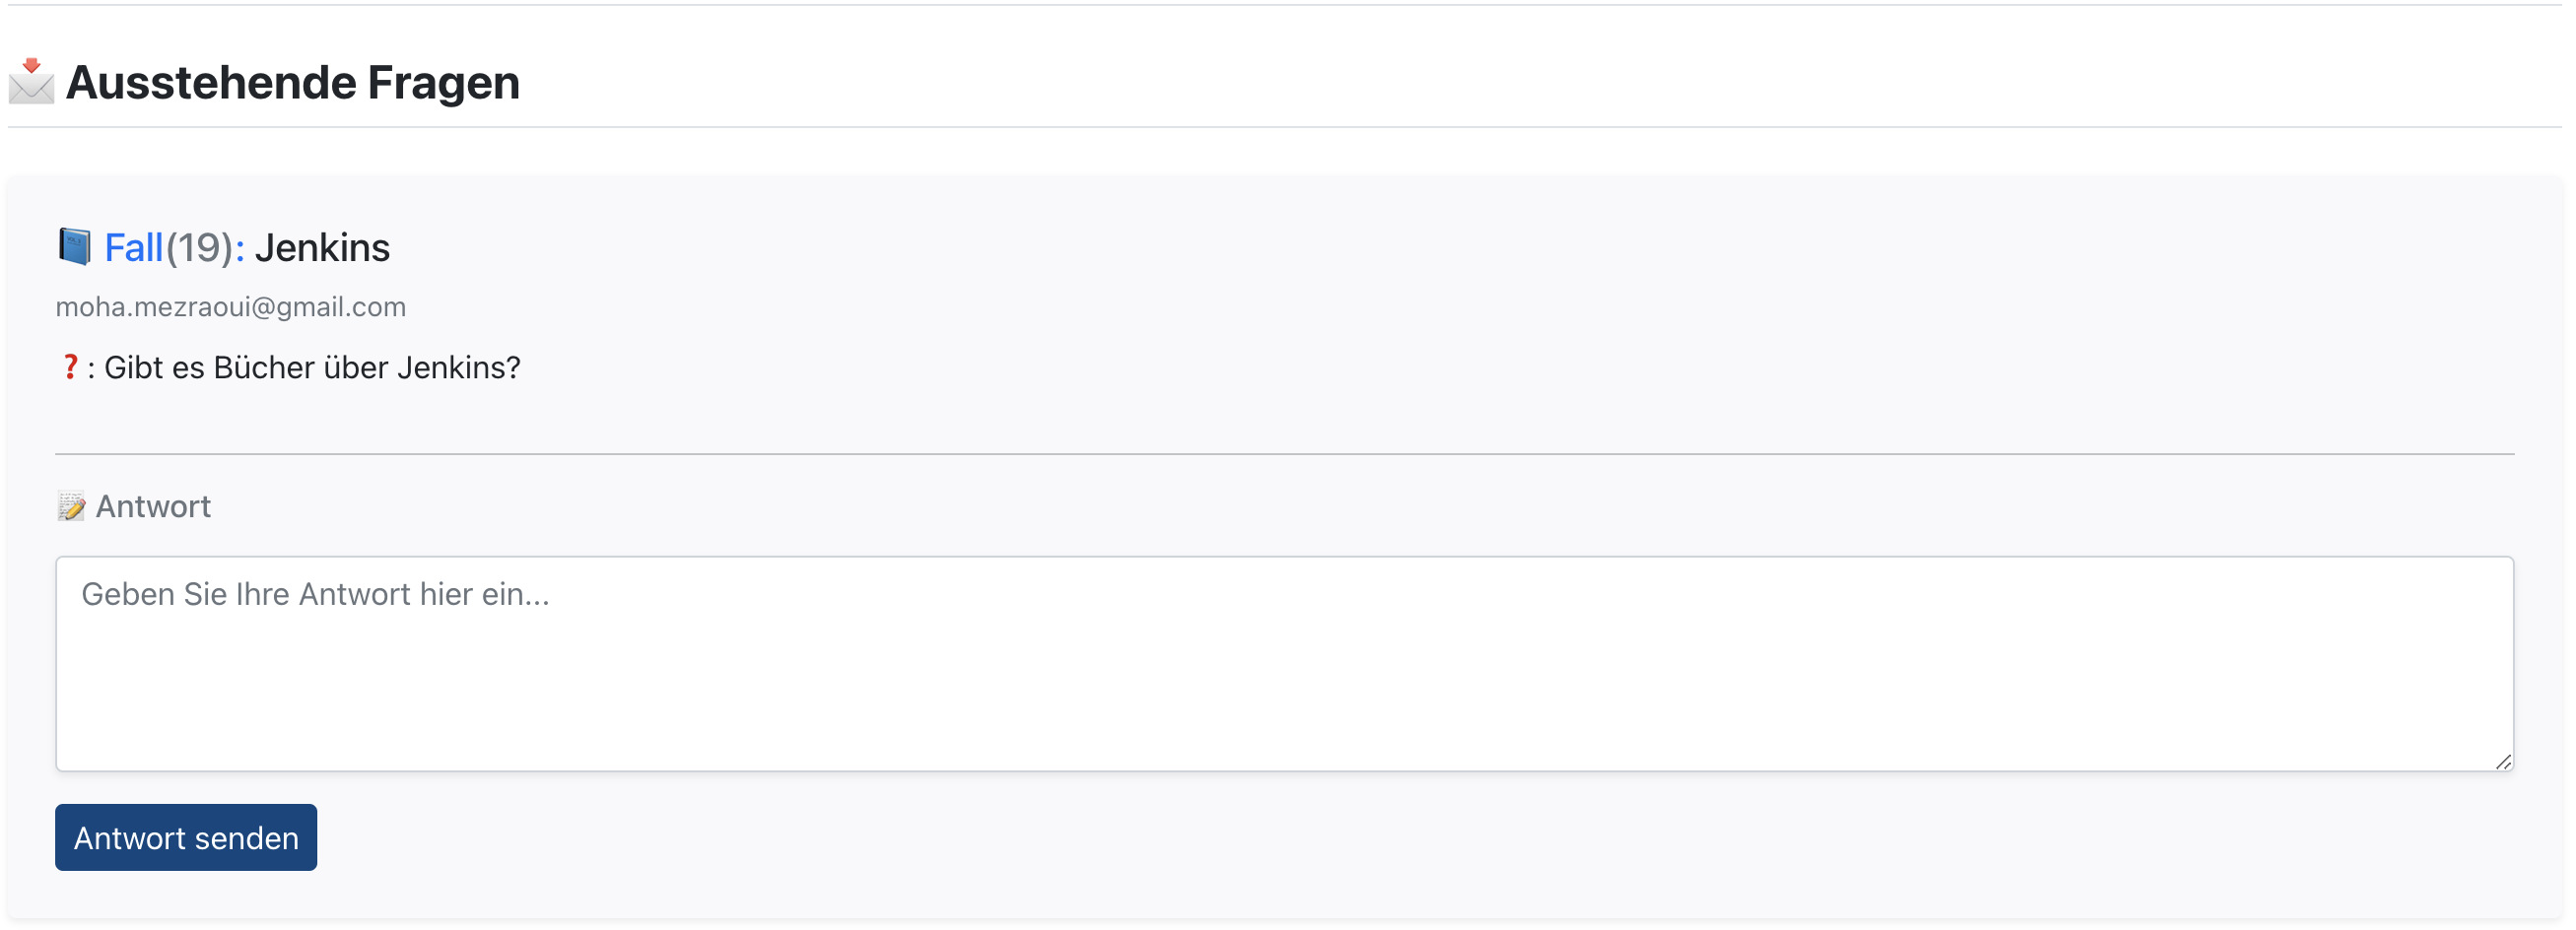
\includegraphics[width=1.0\textwidth]{images/UI-screenshots/Messages-Responses.png}
	\caption{Die Schnittstelle für die Beantwortung von Anfragen}
	\label{fig:Messages-Responses}
\end{figure}




















